\documentclass[12pt, a4paper]{article}
% pacotes utilizados
%\usepackage{abnt-UFPR}
\usepackage[pdftex]{graphicx}
\usepackage{graphicx,url}
\usepackage[utf8]{inputenc}
\usepackage[brazil]{babel}
\usepackage{setspace}
\onehalfspace
\usepackage{enumerate}
\usepackage{multirow}
\usepackage{parskip}
\usepackage{float}
\usepackage{color}
\usepackage[normalem]{ulem}
\usepackage{lmodern}
\usepackage{pdfpages}

\usepackage{listings}

\definecolor{verdao}{rgb}{0.0, 0.5, 0.0}

\lstset{
	language=Python,
	frame=single,
	numbers=left,
	showspaces=false,
	showstringspaces=false,
	basicstyle=\ttfamily,
	captionpos=t,
	basicstyle=\small,
	keywordstyle=\ttfamily \color{blue},
	keywordstyle=[2]\ttfamily \color{blue},
	stringstyle=\color{red}\ttfamily,
	commentstyle=\color{verdao}\ttfamily
}

%\usepackage{fancyhdr}
\usepackage{indentfirst}
\usepackage[a4paper,left=3cm,right=2cm,top=3cm,bottom=2cm]{geometry}
\usepackage[alf]{abntex2cite}
%\pagestyle{headings}
%configuracoes do sumario
\usepackage{tocloft}
\renewcommand{\cftdot}{\textbf{.}}
\renewcommand{\cftsecdotsep}{\cftdotsep}
\renewcommand{\cftsecdotsep}{4}
\renewcommand{\cftsubsecdotsep}{4}
\renewcommand{\cftsecfont}{\normalsize\bfseries}
\renewcommand{\cftsubsecfont}{\normalsize}
\renewcommand{\cftsecpagefont}{\textbf}
\renewcommand{\cftsubsecpagefont}{\textbf}
\cftsetindents{section}{0cm}{1.3cm}
\cftsetindents{subsection}{0cm}{1.3cm}
\cftsetindents{subsubsection}{0cm}{1.3cm}
%\renewcommand{\figurename}{Fig.}
\newcommand{\bigsize}{\fontsize{12pt}{20pt}\selectfont}

\usepackage[labelsep=endash]{caption}
\setlength{\cftsubsecindent}{0em}
\tocloftpagestyle{empty}
\newcommand{\bfemph}[1]{\textbf{\textit{#1}}}
\renewcommand{\emph}[1]{\bfemph{#1}}
%Formatacao de Padroes das Referencias Bibliograficas
%\usepackage{custom-bib}

%Formatacao de Titulos, Secoes, Subtitulos, etc...
\usepackage{titlesec}

\setcounter{secnumdepth}{4}

\titleformat{\section}{\normalfont\normalsize\filright\bfseries}{\thesection}{1em}{\uppercase}
%\renewcommand{\thesubsection}{\alph{subsection}}
\titleformat{\subsection}{\normalfont\normalsize\filright\bfseries}{\thesubsection}{1em}{}
%\renewcommand{\thesubsubsection}{\roman{subsubsection}}
\titleformat{\subsubsection}{\normalfont\normalsize\bfseries}{\thesubsubsection}{1em}{}
%
\titleformat{\paragraph}{\normalfont\normalsize\bfseries}{\theparagraph}{1em}{}
%\titlespacing*{\paragraph}{0pt}{3.25ex plus 1ex minus .2ex}{1.5ex plus .2ex}

%Espacamento de Paragrafos
\setlength{\parindent}{0.8cm}
\setlength{\parskip}{1ex plus 0.5ex minus 0.2ex}
%1ex plus 0.5ex minus 0.2ex
\pagestyle{myheadings}

\pagenumbering{arabic}

\author{ \bf UNIVERSIDADE DO ESTADO DO AMAZONAS - UEA \\[14pt] \small ESCOLA SUPERIOR DE TECNOLOGIA - EST \\[14pt] ENGENHARIA ELÉTRICA \\[96pt] VINICIUS TAVARES COELHO \\[96pt]}
\title{ \rm \bf \Large ANÁLISE DE VIABILIDADE ECONÔMICA E AMBIENTAL DA UTILIZAÇÃO DOS GRUPOS GERADORES DO TRIBUNAL DE CONTAS DO ESTADO DO AMAZONAS ALIMENTADOS POR BIODIESEL PARA GERAÇÃIO DE ENERGIA NA PONTA\\[123pt] \rm \small Manaus \\  2022}


\newcommand{\thesisTitle}{ANÁLISE DE VIABILIDADE ECONÔMICA E AMBIENTAL DA UTILIZAÇÃO DOS GRUPOS GERADORES DO TRIBUNAL DE CONTAS DO ESTADO DO AMAZONAS ALIMENTADOS POR BIODIESEL PARA GERAÇÃO DE ENERGIA NA PONTA}
\newcommand{\thesisAuthor}{VINICIUS TAVARES COELHO}

\pagestyle{myheadings}

% Start the document
\begin{document}

\addtocontents{toc}{\protect\thispagestyle{empty}}
%INÍCIO DA CAPA DA MONOGRAFIA
\thispagestyle{empty}
\begin{center}
\textbf{ UNIVERSIDADE DO ESTADO DO AMAZONAS \\
ESCOLA SUPERIOR DE TECNOLOGIA \\[50pt] }
\textbf{ \\[70pt] {\bigsize VINICIUS TAVARES COELHO} \\[120pt] }
\textbf{ {\bigsize \thesisTitle}  \\[104pt] }
\end{center}
% COMENTÁRIOS DA FOLHA DE ROSTO
\hspace*{8cm}

\vspace*{\fill}

\begin{center}
Manaus \\ 2022
\end{center}

%FIM DA CAPA DA MONOGRAFIA

%INÍCIO DA FOLHA DE ROSTO
\newpage
\thispagestyle{empty}
\begin{center}


% \textbf{ \\[70pt] {\bigsize CARLA PATRICIA MICHILES ARAUJO} \\[120pt] }
\textbf{ {\bigsize \thesisAuthor} \\[120pt] }
\textbf{ {\bigsize \thesisTitle}  \\[50pt] }
\end{center}
% COMENTÁRIOS DA FOLHA DE ROSTO
\hspace*{8cm}
\begin{flushright}
\begin{minipage}{8cm}
\begin{singlespace}
Projeto de pesquisa desenvolvido durante a disciplina de Trabalho de Conclusão de Curso II e apresentada à banca avaliadora do Curso de Engenharia Elétrica da Escola Superior de Tecnologia da Universidade do Estado do Amazonas, como pré-requisito para obtenção do título de Engenheiro Eletricista.\\[50pt]
\end{singlespace}
\end{minipage}
\end{flushright}
\begin{center}
Orientador: Raimundo Cláudio Souza Gomes, Me.

\end{center}

\vspace*{\fill}
\begin{center}
Manaus \\ 2022
\end{center}



%FIM DA FOLHA DE ROSTO

%INICIO DA PAG CATALOGAÇÃO

\newpage
\thispagestyle{empty}

\includepdf[pages=-]{carlaze.pdf}

\newpage
\thispagestyle{empty}
\begin{center}


% \textbf{ \\[30pt] {\bigsize CARLA PATRICIA MICHILES ARAUJO} \\[50pt] }
\textbf{ {\bigsize \thesisAuthor} \\[50pt] }
\textbf{ {\bigsize \thesisTitle}  \\[50pt] }
\end{center}
% COMENTÁRIOS DA FOLHA DE ROSTO
\hspace*{8cm}
\begin{flushright}
\begin{minipage}{8cm}
\begin{singlespace}
Pesquisa desenvolvida durante a disciplina de Trabalho de Conclusão de Curso II e apresentada à banca avaliadora do Curso de Engenharia Elétrica da Escola Superior de Tecnologia da Universidade do Estado do Amazonas, como pré-requisito para obtenção do título de Engenharia Eletricista.\\[30pt]
\end{singlespace}
\end{minipage}
\end{flushright}
\begin{center}
Nota obtida:\uline{\hspace{1cm}}(\uline{\hspace{8cm}})
\vspace{1.0cm}
\begin{center}
Aprovado em 20/05/2022
\end{center}
Área de concentração: Engenharia Elétrica
\end{center}
\vspace{1.2cm}
\begin{center}
BANCA EXAMINADORA
\end{center}
\vspace{1.0cm}

%\begin{flushright}
\begin{minipage}[l]{14cm}
\begin{center}
\hspace{1cm}\uline{\hspace{10.5cm}} \\
\hspace{1cm}Orientador: Raimundo Cláudio Souza Gomes, Me.

\hspace{1cm}\uline{\hspace{10.5cm}} \\
\hspace{1cm}Avaliador: Israel Gondres Torné, Dr.

\hspace{1cm}\uline{\hspace{10.5cm}} \\
\hspace{1cm}Avaliador: Fábio de Sousa Cardoso, Dr.

\end{center}
\end{minipage}

%\end{flushright}
\hspace*{8cm}

\vspace*{\fill}
\begin{center}
Manaus\\2017
\end{center}



\newpage
\thispagestyle{empty}
\begin{flushright}
\begin{minipage}{8cm}
\begin{singlespace}
{\begin{center}\vspace{18cm}\textbf{\normalsize Dedicatória}\vspace{36pt}\end{center}}
Dedico este trabalho ao meu avô José Rodrigues (in memorian), que me ensinou o valor do trabalho.\\[50pt]
\end{singlespace}
\end{minipage}
\end{flushright}
\newpage
\thispagestyle{empty}
\vspace*{4.5cm}
{\begin{center}\textbf{\normalsize AGRADECIMENTO}\vspace{36pt}\end{center}}
\hspace*{0.8cm}À Deus, que tornou possível, mesmo com muitos sacrifícios me deu fé para finalização deste trabalho.

\hspace*{0.8cm} Agradeço á minha família, que sempre proporcionaram condições adequadas para crescer na vida pessoal e profissional e ao meu noivo, amigo e compaheiro de todas as horas, Kenny Vinente, pelo carinho, paciência, compreensão e amor.

\hspace*{0.8cm} Agradeço ao meu orientador, Wheidima Carneiro de Melo, por fornecer todo o apoio que eu precisava para a realização deste trabalho.


\hspace*{0.8cm}Aos engenheiros, Thales Araujo, Ronald Santos e Adriano Ibrahim, pelo tempo dedicado na empresa Philips, que contribuiram com material e suporte no entendimento teórico do sinal do eletrocardiograma.


\hspace*{0.8cm}Aos alunos de graduação, Giovanni Antonnacio e Marcus Vinícius pelo suporte no desenvolvimento do projeto e aos Notáveis que estiveram ao meu lado me incentivando durante todo o processo.




\newpage

\thispagestyle{empty}
\vspace*{4cm}
{\begin{center}\textbf{\normalsize RESUMO}\vspace{36pt}\end{center}}
O presente trabalho tem como objetivo desenvolver um protótipo de eletrocardiógrafo portátil de baixo custo que realize a aquisição e transmissão dos sinais ECG em tempo real. Sua apresentação está dividida em quatro capítulos. O primeiro capítulo, Referencial Teórico, apresenta assuntos referente a composição do eletrocardiograma, necessárias para o desenvolvimento deste trabalho, o coração, o ciclo cardíaco, o eletrocardiograma, derivações eletrocardiográficas, o triângulo de einthoven, eletrodos e interferência em sinais de ECG. O segundo capítulo, Metodologia, apresenta os materias e métodos necessário para aquisição e transmissão dos sinais de ECG. O terceiro capítulo, Implementação do Projeto, descreve o uso dos componentes, assim como o desenvolvimento do hardware utilizando a placa de aquisição e o Rapsberry Pi 3, além de descrever o uso dos protocolos utilizados, o funcionamento da arquitetura cliente-servidor para transmissão de dados utilizando a rede Wi-Fi como meio de comunicação. O quarto capítulo apresenta os resultados obtidos durante o desenvolvimento do projeto. Apesar do estudo ter um caráter de implementação do circuito de aquisição ECG, os resultados obtidos apresentaram ruídos nas formas de ondas, que poderiam ser diminuídos se algoritmos específicos com certo grau de complexidade fossem utilizados para realizar a separação do sinal e ruído. Nas conclusões são apresentadas as dificuldades enfrentadas na realização deste projeto, os objetivos que foram alcançados e aplicações para o protótipo desenvolvido.


\textbf{Palavras chave}: eletrocardiograma. protótipo de baixo custo, Raspberry Pi 3

\newpage
\thispagestyle{empty}
\vspace*{4.4cm}
{\begin{center}\textbf{\normalsize ABSTRACT}\vspace{36pt}\end{center}}
The present work aims to develop a prototype of a low cost portable electrocardiograph that performs the acquisition and transmission of ECG signals in real time. Its presentation is divided into four chapters. The first chapter, Theoretical Framework, presents subjects related to the composition of the electrocardiogram necessary for the development of this work, the heart, the cardiac cycle, the electrocardiogram, electrocardiographic leads, the eithoven’s triangle, electrodes and interference on ECG signals. The second chapter, Methodology, presents the materials and methods necessary for the acquisition and transmission of ECG signals. The third chapter, Project Implementation, describes the use of the components, as well as hardware development using the acquisition board and a Rapsberry Pi 3. In addition, it is described the protocols used and the operation of the client-server architecture for data transmission using the wireless network to communicate them. The fourth chapter presents the results obtained during the development of the project. Although the study focused on the implementation of an ECG acquisition circuit, the results obtained presented noises in the waveforms, which could be reduced if specific algorithms with a certain degree of complexity were used to perform signal and noise separation. Finally, the conclusion presents the challenges faced in the accomplishment of this project, the objectives achieved and applications for the developed prototype.


\textbf{Keywords}: electrocardiogram, low cost prototype, Rapsberry Pi 3


%INÍCIO DA LISTA DE FIGURAS

\newpage
\pagestyle{empty}
%\vspace*{4cm}
\listoffigures
\clearpage

%FIM DA LISTA DE FIGURAS



%INÍCIO DO SUMÁRIO
\newpage
\pagestyle{empty}
%\vspace*{3.5cm}
\renewcommand{\contentsname}{\begin{center}\textbf{\normalsize SUMÁRIO}\vspace{36pt}\end{center}}
\tableofcontents
\clearpage
%FIM DO SUMÁRIO

\pagestyle{myheadings}

\newpage
%\vspace*{4cm}
\setcounter{page}{12}
\begin{center}
\section{INTRODUÇÃO}
%\textbf{INTRODUÇÃO\\\\}
\end{center}
\par
%\addcontentsline{toc}{section}{INTRODUÇ\~AO}	

	\hspace{0.8cm}Devido à forte crise do setor elétrico dos últimos anos, os consumidores brasileiros de energia elétrica têm convivido com sucessivos aumentos tarifários e sofrido com inúmeras falhas no fornecimento, principalmente, durante os horários de maior consumo \cite{kurek}. Agora, os consumidores, particularmente, do setor produtivo, passam a ver as ameaças de racionamento e black-outs de energia com sério risco de se tornarem realidade. 
    
    Com essa crescente perda de confiabilidade do sistema de fornecimento de energia, muitas empresas têm utilizado grupos geradores como fonte backup de energia, a fim de evitar paradas e garantir a continuidade dos processos produtivos, mesmo em meio aos incidentes de falta de energia. Nesse cenário, a demanda por geradores movidos a diesel tem crescido significativamente e fabricantes relatam alta de até 35\% nos pedidos e cotações por geradores a diesel e a gás \cite{fucuchima}.
    
    Entretanto, limitar o uso desses equipamentos somente a este fim, implica numa subutilização de recurso, que leva ao questionamento sobre a validade do investimento. 
   
    Com o aumento das tarifas, especialmente nos horários de ponta, o uso de grupos geradores se apresenta como uma alternativa plausível para atuar na cobertura de picos de carga e, assim, evitar o custo por incidência das altas penalidades (sob tarifas ainda mais caras) aplicadas pelas concessionárias àqueles que violam os limites estabelecidos em contrato. Mesmo em horários de baixo consumo, os grupos geradores podem oferecer alternativa de menor custo na geração de energia elétrica, principalmente, se abastecidos com combustíveis mais baratos.
    
    Este trabalho apresenta um estudo de caso das instalações do Tribunal de Contas do Estado do Amazonas (TCE -- AM), com o objetivo de realizar um levantamento do atual estado das instalações e recursos de geração de energia, visando descrever um método para implementar a utillização dos grupos geradores já presentes na unidade de forma ativa, para geração de energia na ponta, utilizando o Biodiesel como biocombustível, aferindo a viabilidade econômica e ambiental desse esforço.
    
\subsection{TEMA}
\subsubsection{Delimitação do tema}

\subsection{PROBLEMA DE PESQUISA}

    \hspace{0.8cm}Num cenário de crescente crise no sistema energético brasileiro, empresas de diversos setores tem manifestado interesse na busca de soluções alternativas que possibilitem a redução dos gastos com energia elétrica. Nesse contexto, muitas empresas utilizam grupos geradores como fonte backup na prevenção de paralizações por falta de energia. Entretanto, limitar o uso desses equipamentos somente a este fim, implica numa subutilização de recurso, que leva ao questionamento sobre a validade do investimento. 
    
    Com o aumento das tarifas, especialmente nos horários de ponta, o uso de grupos geradores se apresenta como uma alternativa plausível para atuar na cobertura de picos de carga e, assim, evitar o custo por incidência das altas penalidades (sob tarifas ainda mais caras) aplicadas pelas concessionárias àqueles que violam os limites estabelecidos em contrato. Mesmo em horários de baixo consumo, os grupos geradores podem oferecer alternativa de menor custo na geração de energia elétrica, principalmente, se abastecidos com combustíveis mais baratos.
    
    No entanto, o sucesso na implementação dessa estratégia depende diretamente do custo em um investimento contínuo: o combustível diesel. Com a alta nos preços do petróleo, o preço desse combustível vem aumentando numa escala superior ao da inflação nos últimos anos. De acordo com a pesquisa da Vale Card, uma empresa especializada em soluções de gestão de frotas, o preço médio do diesel comum subiu 25,26\% neste período. Já a inflação teve uma variação de 18,42\%. \cite{janone}. 
    
    Nesse contexto, a utilização do Biodiesel, uma fonte renovável de energia, pode ser uma alternativa para alimentação dos grupos geradores não só de menor custo como menos poluente e de baixo impacto ao meio ambiente. Este trabalho propõe a utillização do biodiesel como combustível dos grupos geradores, aplicando-os de forma ativa para redução de custos de energia elétrica.


\subsection{OBJETIVOS}
\subsubsection{Objetivo geral}
\subsubsection{Objetivos específicos}

\subsection{JUSTIFICATIVA}

A pesquisa propõe uma alternativa de utilização dos grupos geradores, primariamente utilizados como fonte reserva de energia, para trazer economias nas tarifas pagas e redução de custos, frente ao cenário de crise energética e aumento significativo nas tarifas de consumo de energia elétrica, tendo como objeto de estudo as instalações do Tribunal de Contas do Estado do Amazonas.

Para isso, propõe-se a utilização do biodiesel como combustível dessas máquinas geradoras, que é uma fonte de energia renovável e de menor custo em comparação ao diesel convencional de origem fóssil. Além de baratear a utilização dos grupos geradores, a proposta tem grande potencial de redução de emissão de poluentes. Segundo a \citeonline{embrapa}, uma mistura de 20\% de biodiesel em diesel fóssil reduz em 70\% a emissão de gases do efeito estufa.


\subsection{METODOLOGIA}

\subsection{ESTRUTURA DO TRABALHO}

Este trabalho foi dividido nos seguintes capítulos:

\begin{itemize}
    \item    Capíutlo 1: Introdução do trabalho, abordando o tema e sua delimitação, o problema de pesquisa abordado, os objetivos da pesquisam justificativas e metodologia proposta.
    \item Capíutlo 2: 
    \item Capíutlo 3
    \item Capíutlo 4
    \item Capíutlo 5
\end{itemize}

   
    
    

\section{REFERENCIAL TEÓRICO}	

\subsection{O BIODIESEL}
\hspace*{0.8cm}Biodiesel é uma denominação abrangente de combustíveis e aditivos provenientes de fontes renováveis. Um combustível que pode ser utilizado em substituição ao diesel comum, sem proporcionar danos mecânicos ao equipamento, além de possuir desempenho de igual qualidade em relação à potência, rendimento, etc. (BUMBA E YAMAMURA, 2015).

\begin{figure}[!htb]
\begin{center}
			\caption{Principais matérias primas para produção de biodiesel}
			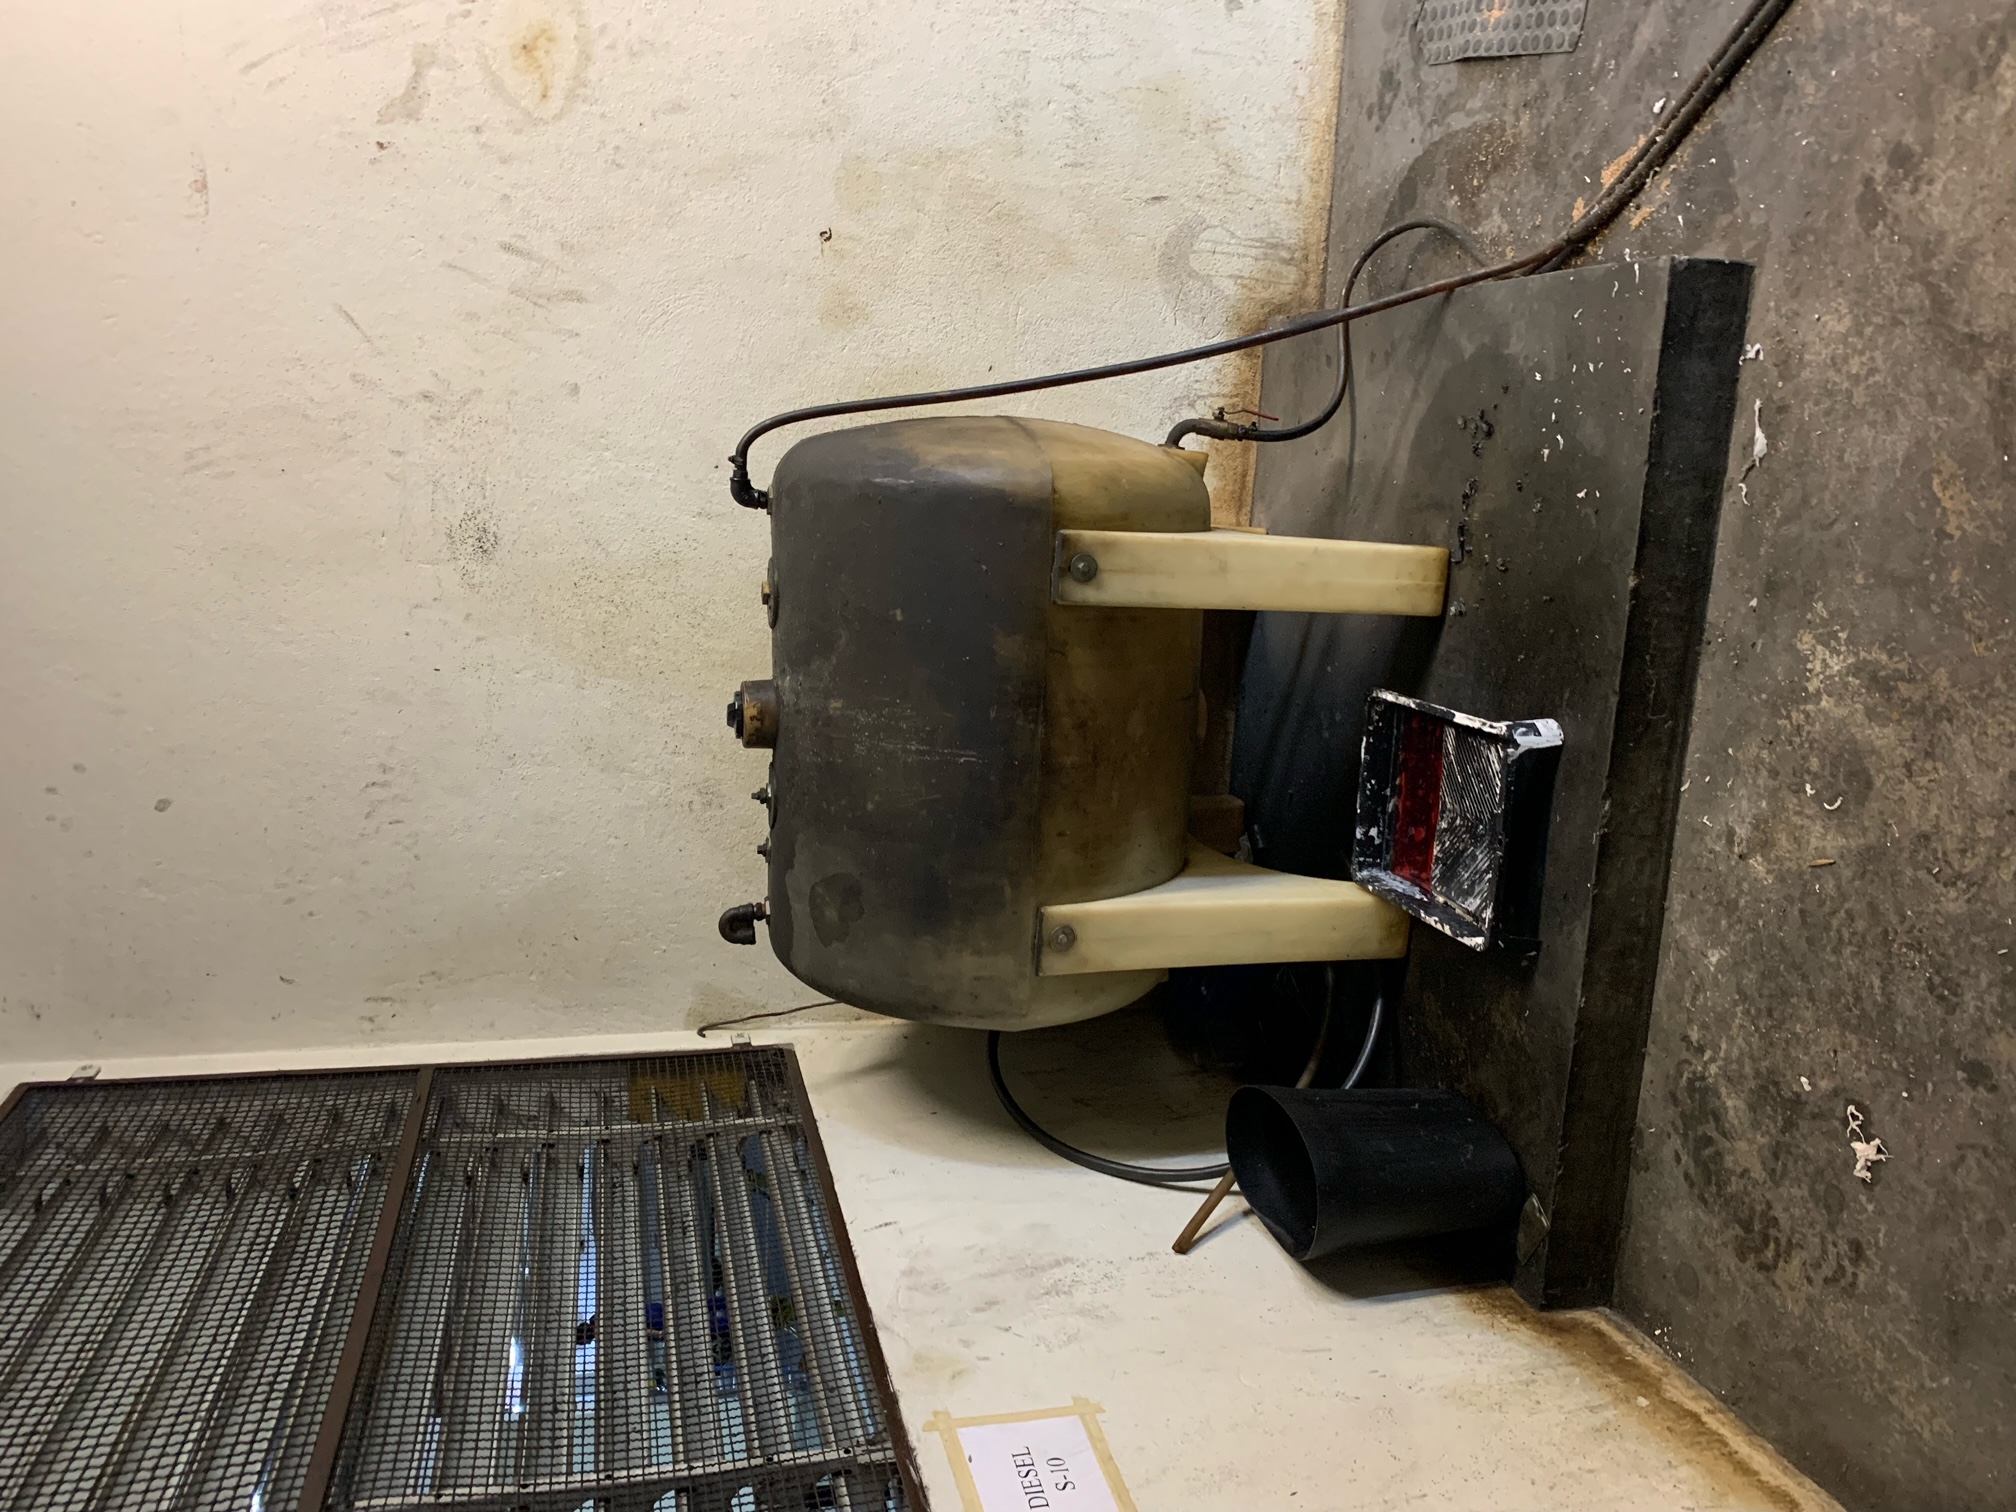
\includegraphics[width=.9\textwidth]{Figuras/image0.jpeg}
            \vspace*{\fill} 
            \begin{quote} 
            \centering 
            Fonte: Própria.
            \end{quote}
            \vspace*{\fill}
			\label{fig:ramcor}
\end{center}
\end{figure}

    O biodiesel pode ser produzido a partir de várias matérias-primas diferentes. É possível obter o combustível partindo de óleos vegetais, gorduras animais ou produtos residuais, como o óleo de fritura já usado. \cite{biodieselbr}.
    
    Importante ressaltar que o biodiesel não é só um produto nascido da necessidade de adaptações ou reciclagem. É um combustível de qualidade que pode ser utilizado em qualquer motor a diesel, com pouca ou nenhuma necessidade de adaptação, por vezes demonstrando desempenho até superior ao combustível padrão (DIAS, 2007).
    
\subsubsection{Impactos ambientais da substituição do Diesel mineral pelo Biodiesel}
    
\subsubsection{Utilização de Biodiesel em grupos geradores a Diesel}

\hspace{0.8cm}Assim como o diesel mineral, o biodiesel opera em motores de combustão-ignição. Pode ser usado como um substituto, mistura ou aditivo ao óleo diesel. Misturas de até 20\% de biodiesel (a 80\% de diesel convencional) podem ser usadas em praticamente qualquer equipamento diesel e são compatíveis com a maioria dos equipamentos de armazenamento e distribuição. Tais misturas (20\% ou menos) não requerem nenhuma modificação de motor e podem proporcionar performances próximas às do diesel. Misturas mais elevadas, ou até o biodiesel puro (100\% biodiesel, ou B100), podem ser usadas em muitos motores com pequenas alterações, posto que as propriedades físicas do Biodiesel são muito semelhantes às do Diesel. \cite{udaeta}

\subsubsection{O BIODIESEL A PARTIR DE ÓLEOS RESIDUAIS DE FRITURAS}

\hspace*{0.8cm}Atualmente, como não há uma legislação específica para o descarte de óleos residuais, muitos estabelecimentos descartam o óleo de fritura de forma inadequada, como por exemplo na rede de esgoto. Tal forma de descarte, resulta no entupimento de tubulações e consequente utilização de produtos químicos para desentupir as tubulações, produtos estes que são tóxicos e ocasionam danos ambientais juntamente com o óleo. \cite{bumba}.

    Sabe-se que um litro de óleo pode contaminar 1 milhão de litros de água, quantidade esta suficiente para o consumo de uma pessoa durante 14 anos. Uma vez presente no meio ambiente de forma inadequada, o óleo, de menor densidade que a água,  permanece  na  superfície, criando uma barreira que dificulta a entrada de luz e a oxigenação, comprometendo assim a base da cadeia alimentar aquática. \cite{bilck}.
    
    Além da contaminação das águas, o óleo que atinge o leito de rios o impermeabiliza, favorecendo enchentes. \cite{felizardo}.

    Há três vantagens principais de se utilizar óleos residuais de frituras como matéria prima para a produção de biodiesel: a) no âmbito tecnológico, com a não necessidade do processo de extração do óleo; b) no âmbito econômico, devido à diminuição do custo da matéria prima com o resíduo de fritura; c) no âmbito ambiental, pois destina-se adequadamente um resíduo que em geral é descartado inadequadamente no meio ambiente. \cite{bumba}.

\subsection{CLASSIFICAÇÃO DOS CONSUMIDORES}

\subsubsection{Consumidor grupo B}

Consumidor do grupo B é aquele que recebe energia elétrica na tensão entre 220 e 380 V e tem com a concessionária de energia um contrato de adesão. Contrato de adesão é um instrumento contratual, com cláusulas vinculadas às normas e regulamentos aprovados pela ANEEL, não podendo o conteúdo das mesmas ser modificado pela concessionária ou consumidor, a ser aceito ou rejeitado de forma integral.

Os consumidores do Grupo B (baixa tensão -- $<$ 2.300 Volts) são classificados em:

\begin{itemize}
    \item B1 -- residencial;
    \item B2 -- rural;
    \item B3 -- demais classes; e
    \item B4 -- iluminação pública.
\end{itemize}

Os consumidores de baixa tensão (Grupo B) são classificados ainda de acordocom o número de fases. São três os tipos de fornecimento, conforme o número de fases:

\begin{itemize}
    \item Tipo A -- monofásico – dois condutores (uma fase e o neutro);
    \item Tipo B -- bifásico – três condutores (duas fases e o neutro); e
    \item Tipo C -- trifásico – quatro condutores (três fases e o neutro).
\end{itemize}

Para determinação destes, deverá ser calculada a carga instalada de cada unida-
de consumidora. Esta carga será o somatório das potências nominais de placa
dos aparelhos elétricos e das potências de iluminação declaradas.
Quando houver cargas de motores, deverão ser computadas as suas respectivas
quantidades e potências individuais. \cite{procel}.

\begin{figure}[!htb]
\begin{center}
			\caption{ Instalação elétrica residencial}

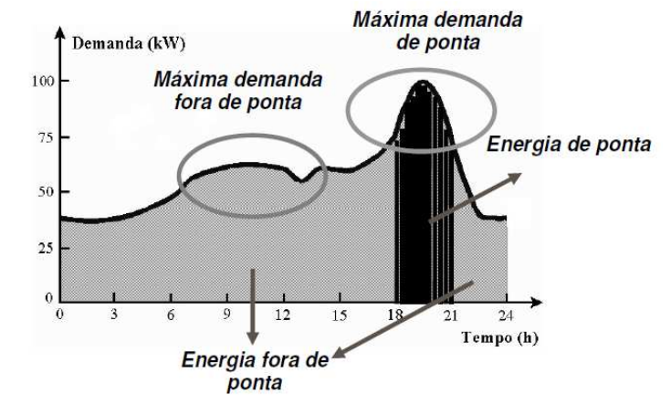
\includegraphics[width=.9\textwidth]{Figuras/ponta.png}
            \vspace*{\fill} 
            \begin{quote} 
            \centering 
            Fonte: \cite{procel}
            \end{quote}
            \vspace*{\fill}
			\label{fig:instres}
\end{center}
\end{figure}

Observando o funcionamento de uma instalação elétrica residencial, comercial
ou industrial, pode-se constatar que a potência elétrica consumida é variável a
cada instante. Isto ocorre porque nem todas as cargas instaladas estão todas em
funcionamento simultâneo. A potência total solicitada pela instalação da rede a
cada instante será, portanto, função das cargas em operação e da potência elé-
trica absorvida por cada uma delas a cada instante. \cite{procel}.

\subsubsection{Consumidor grupo A}

São os consumidores de alta tensão (tensão maior ou igual a 2.300 volts). \cite{procel}.

Para cargas com potência superior a 75kW é inconveniente para a concessionária realizar a alimentação de energia em baixa tensão, pois teria que construir subestações em via pública e instalar cabos de grande capacidade de corrente em propriedades particulares (empresas). \cite{procel}.

Define-se uma subestação como um conjunto de aparelhos e equipamentos destinados a modificar as características da energia elétrica (tensão e corrente), permitindo a sua distribuição aos pontos de consumo em níveis adequados de utilização. \cite{procel}.

Subestação do consumidor é aquela construída em propriedade particular suprida através de alimentadores de distribuição primários originados da concessionária. A partir da subestação a concessionária fará o fornecimento em tensão primária de 15 ou 25 kV. \cite{procel}.

Os consumidores do grupo A (média tensão = 2,3 kV até 69 kV) são classificados em:

\begin{itemize}
    \item A3 - 69 kV
    \item A3a -30 kV a 44 kV – normal 34,5kV
    \item A4 - 2,3 kV a 25 kV – normal 13,8kV
    \item AS - sistemas subterrâneos
\end{itemize}

\subsection{ESTRUTURA TARIFÁRIA}

\subsubsection{O horário de ponta}

\paragraph{test}

\hspace*{0.8cm}O  horário  de  ponta  é  o  período  de  três  horas  consecutivas  exceto  sábados, domingos e feriados nacionais no qual o consumo de energia elétrica está em seu ápice. 
    Nesse  período  a  tarifa  praticada  pela  concessionária  de  energia  aumenta consideravelmente,  pois  há  uma  elevação  do  consumo  em  nível  nacional, sobrecarregando os sistemas de geração, transmissão e distribuição. Esse período de três horas  é  definido  pela  concessionária  em  função  das  características  de  seu  sistema elétrico,  sendo  os  valores  máximos  atingidos  entre  as  17  e  22  horas. \cite{costa}

\begin{figure}[!htb]
\begin{center}
			\caption{Características da curva de carga diária de um consumidor genérico.}

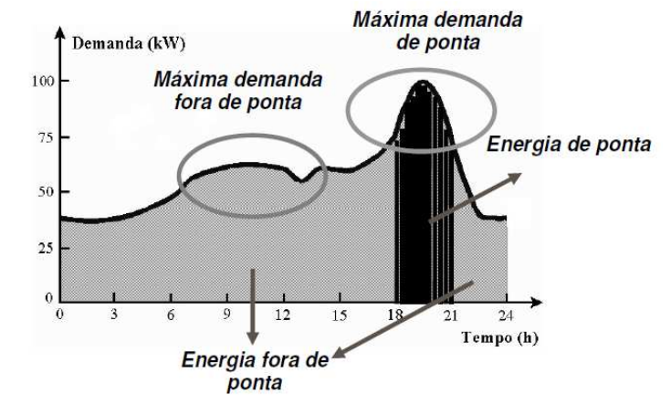
\includegraphics[width=.9\textwidth]{Figuras/ponta.png}
            \vspace*{\fill} 
            \begin{quote} 
            \centering 
            Fonte: \cite{procel}
            \end{quote}
            \vspace*{\fill}
			\label{fig:ponta}
\end{center}
\end{figure}

Gerar  energia  para  consumo  no  horário  de  ponta  tem  o  inconveniente  da  necessidade  de trocar a  fonte  supridora  duas  vezes  por  dia,  no início e ao término  do  período,  nos  dias  úteis.  Embora  a  transferência  de  carga  possa  ser  feita  rapidamente,  haverá interrupção do suprimento de energia, o que poderá ser inaceitável para algumas  atividades que não estejam protegidas por fontes de energia segura. Para solucionar este inconveniente,  pode-se  dotar  o(s)  grupo(s)  gerador(es)  com  sistemas  de  transferência  em transição fechada, sem interrupção e passagem da carga de uma para outra fonte em  rampa suave. Entretanto, para isso é necessário operar instantaneamente na condição de  paralelismo com a rede da concessionária. \cite{costa}
\section{ANÁLISE DAS INSTALAÇÕES DO TCE-AM} % 296 lines

\hspace*{0.8cm}Este capítulo aborda as instalações do Tribunal de Contas do Estado do Amazonas, suas características de carga demandada e as máquinas de geração de energia que se encontram instaladas nas dependências do 

O objetivo desta análise foi adquirir as informações técnicas pertinentes ao funcionamento dos grupos geradores, suas especificações de conversão, a fim de estimar o potencial de geração de energia.

Com estes dados, foi possível analisar as possíveis adaptações necessárias para operar estes equipamentos utilizando o biodiesel como combustível.

A segunda parte do projeto consistiu no estudo das adaptações necessárias para que estes equipamentos possam operar utilizando o biodiesel como combustível, e, na sequência, a análise das implicações dessa mudança.

A unidade conta com um grupo gerador cuja potência aparente é de 750 kVA que atende os dois prédios principais, enquanto um segundo gerador, de potência aparente 450 kVA, atende o prédio anexo, que fica na parte de trás das dependências. 
    
\begin{figure}[H]
\begin{center}
			\caption{Entrada da subestação do TCE-AM}
			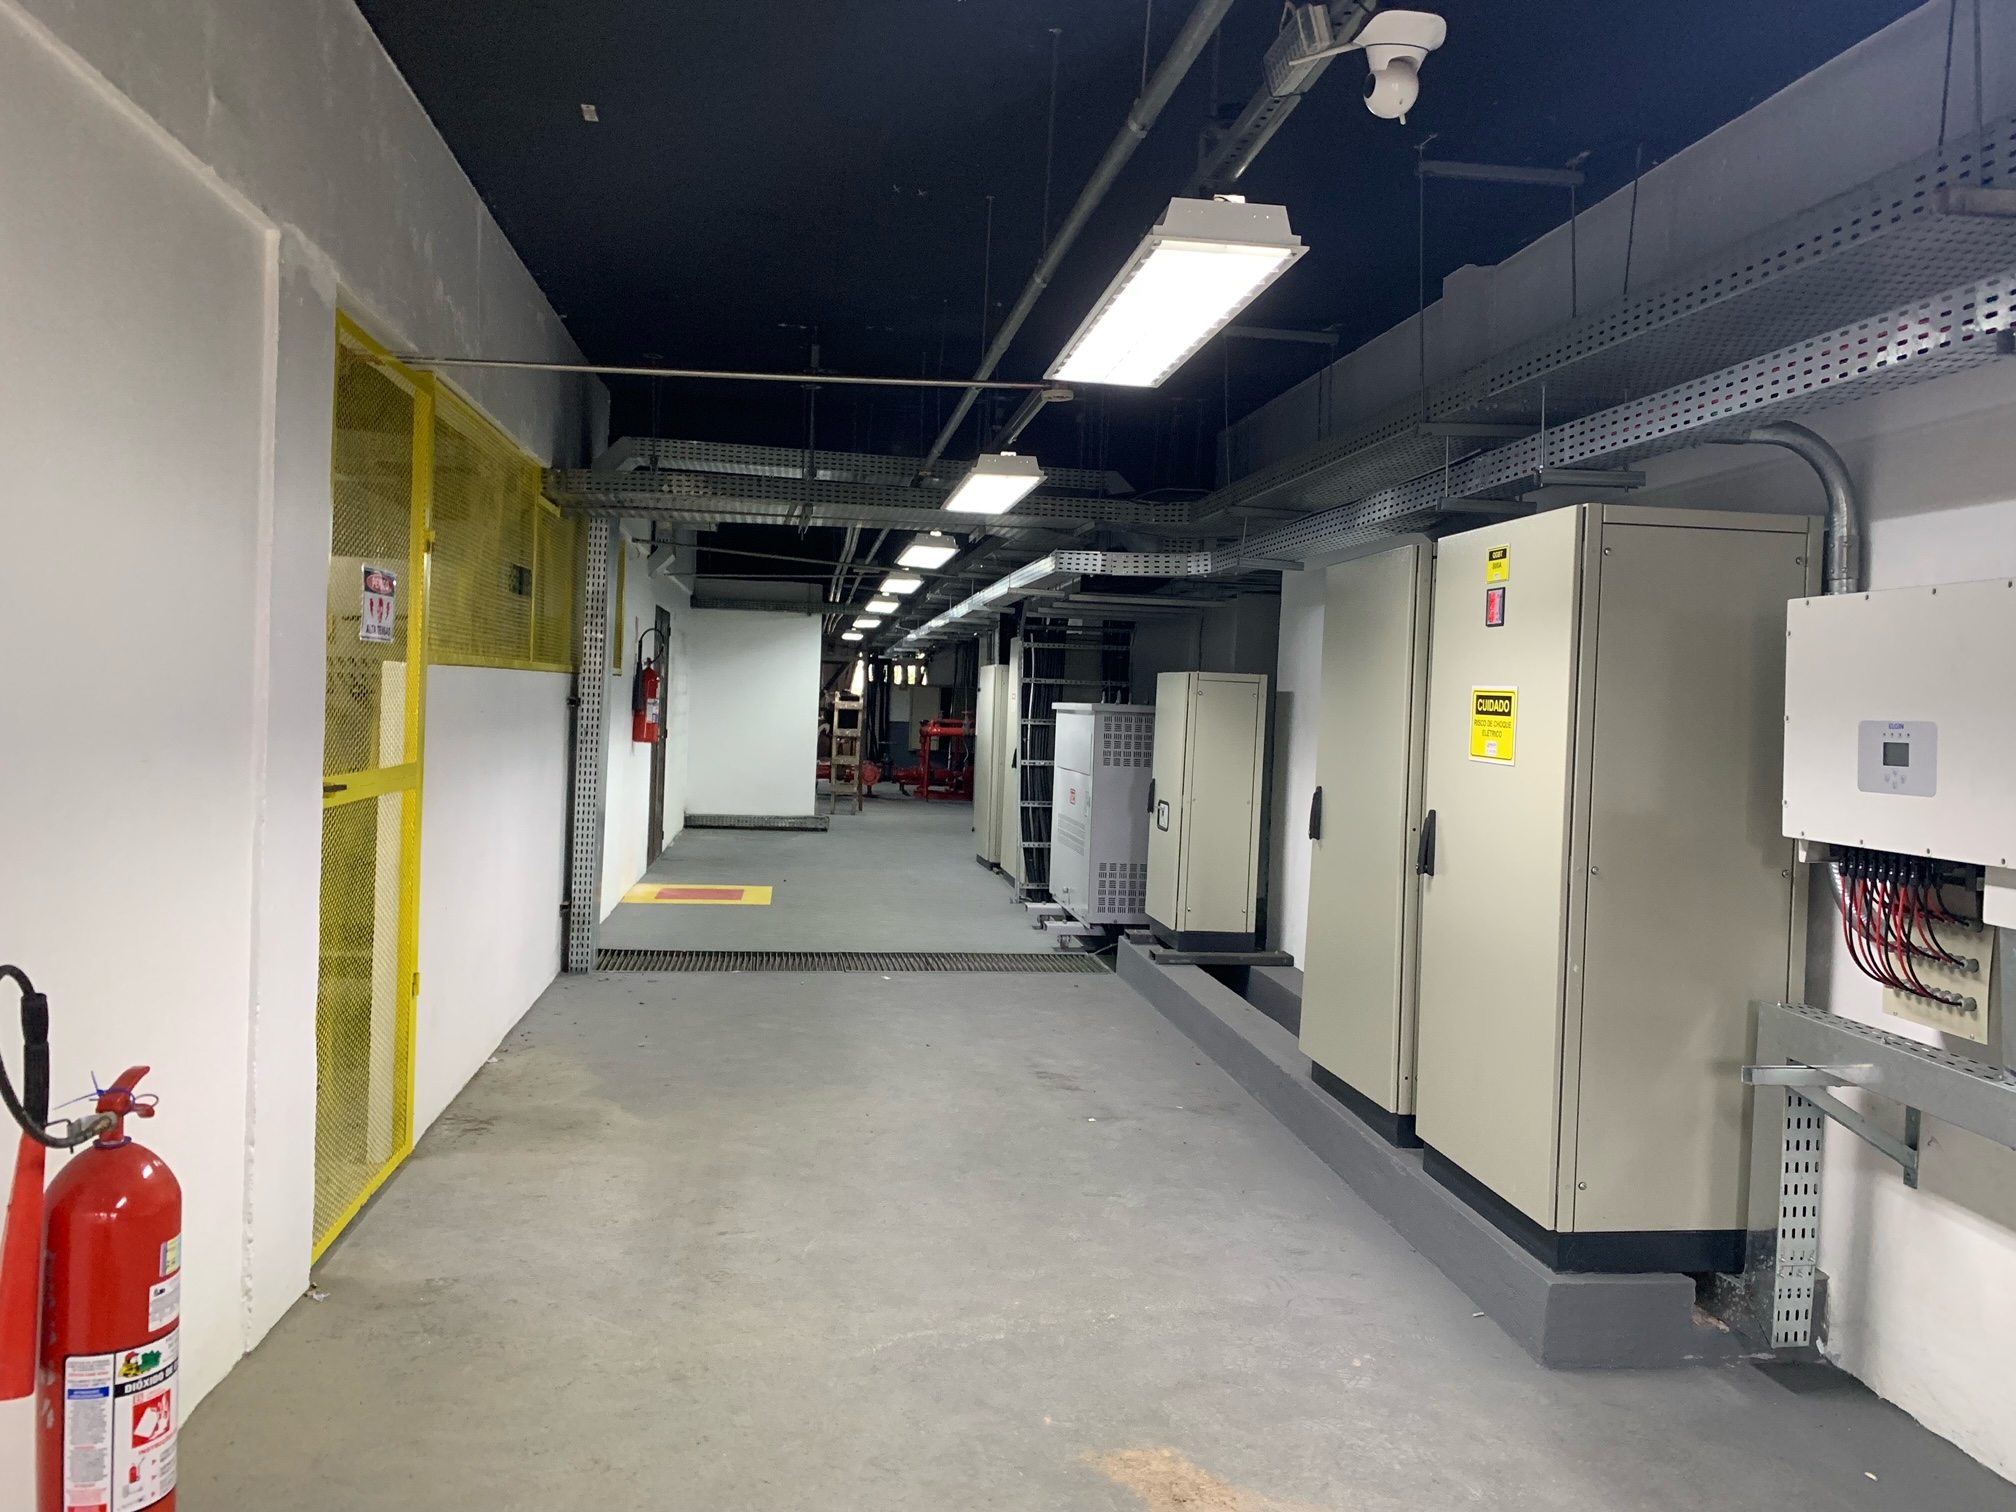
\includegraphics[width=.9\textwidth]{Figuras/deps.jpeg}
            \vspace*{\fill} 
            \begin{quote} 
            \centering 
            Fonte: própria.
            \end{quote}
            \vspace*{\fill}
			\label{fig:tceinst}
\end{center}
\end{figure}

Há, ainda, um terceiro grupo gerador, de 125 kVA, que atua somente como \textit{backup}, em caso de falha do primeiro. A razão para isto é que os prédios principais abrigam a Secretaria de Tecnologia da Informação (Setin), que conta com um Data Center, e este último gerador o alimenta exclusivamente.

A Figura \ref{fig:tceinst} mostra um panorama geral da subestação que se encontra no prédio principal e comporta o grupo gerador principal da unidade.

\subsection{Grupo gerador prédio principal}
\hspace*{0.8cm} O Grupo gerador principal (Figura \ref{fig:gerador750}) tem como responsabilidade atender os dois prédios principais da unidade. É importante resasltar que no momento da realização do estudo esse equipamento não atendia 100\% da unidade.

\begin{figure}[H]
\begin{center}
			\caption{Grupo gerador principal de 750 kVA}
			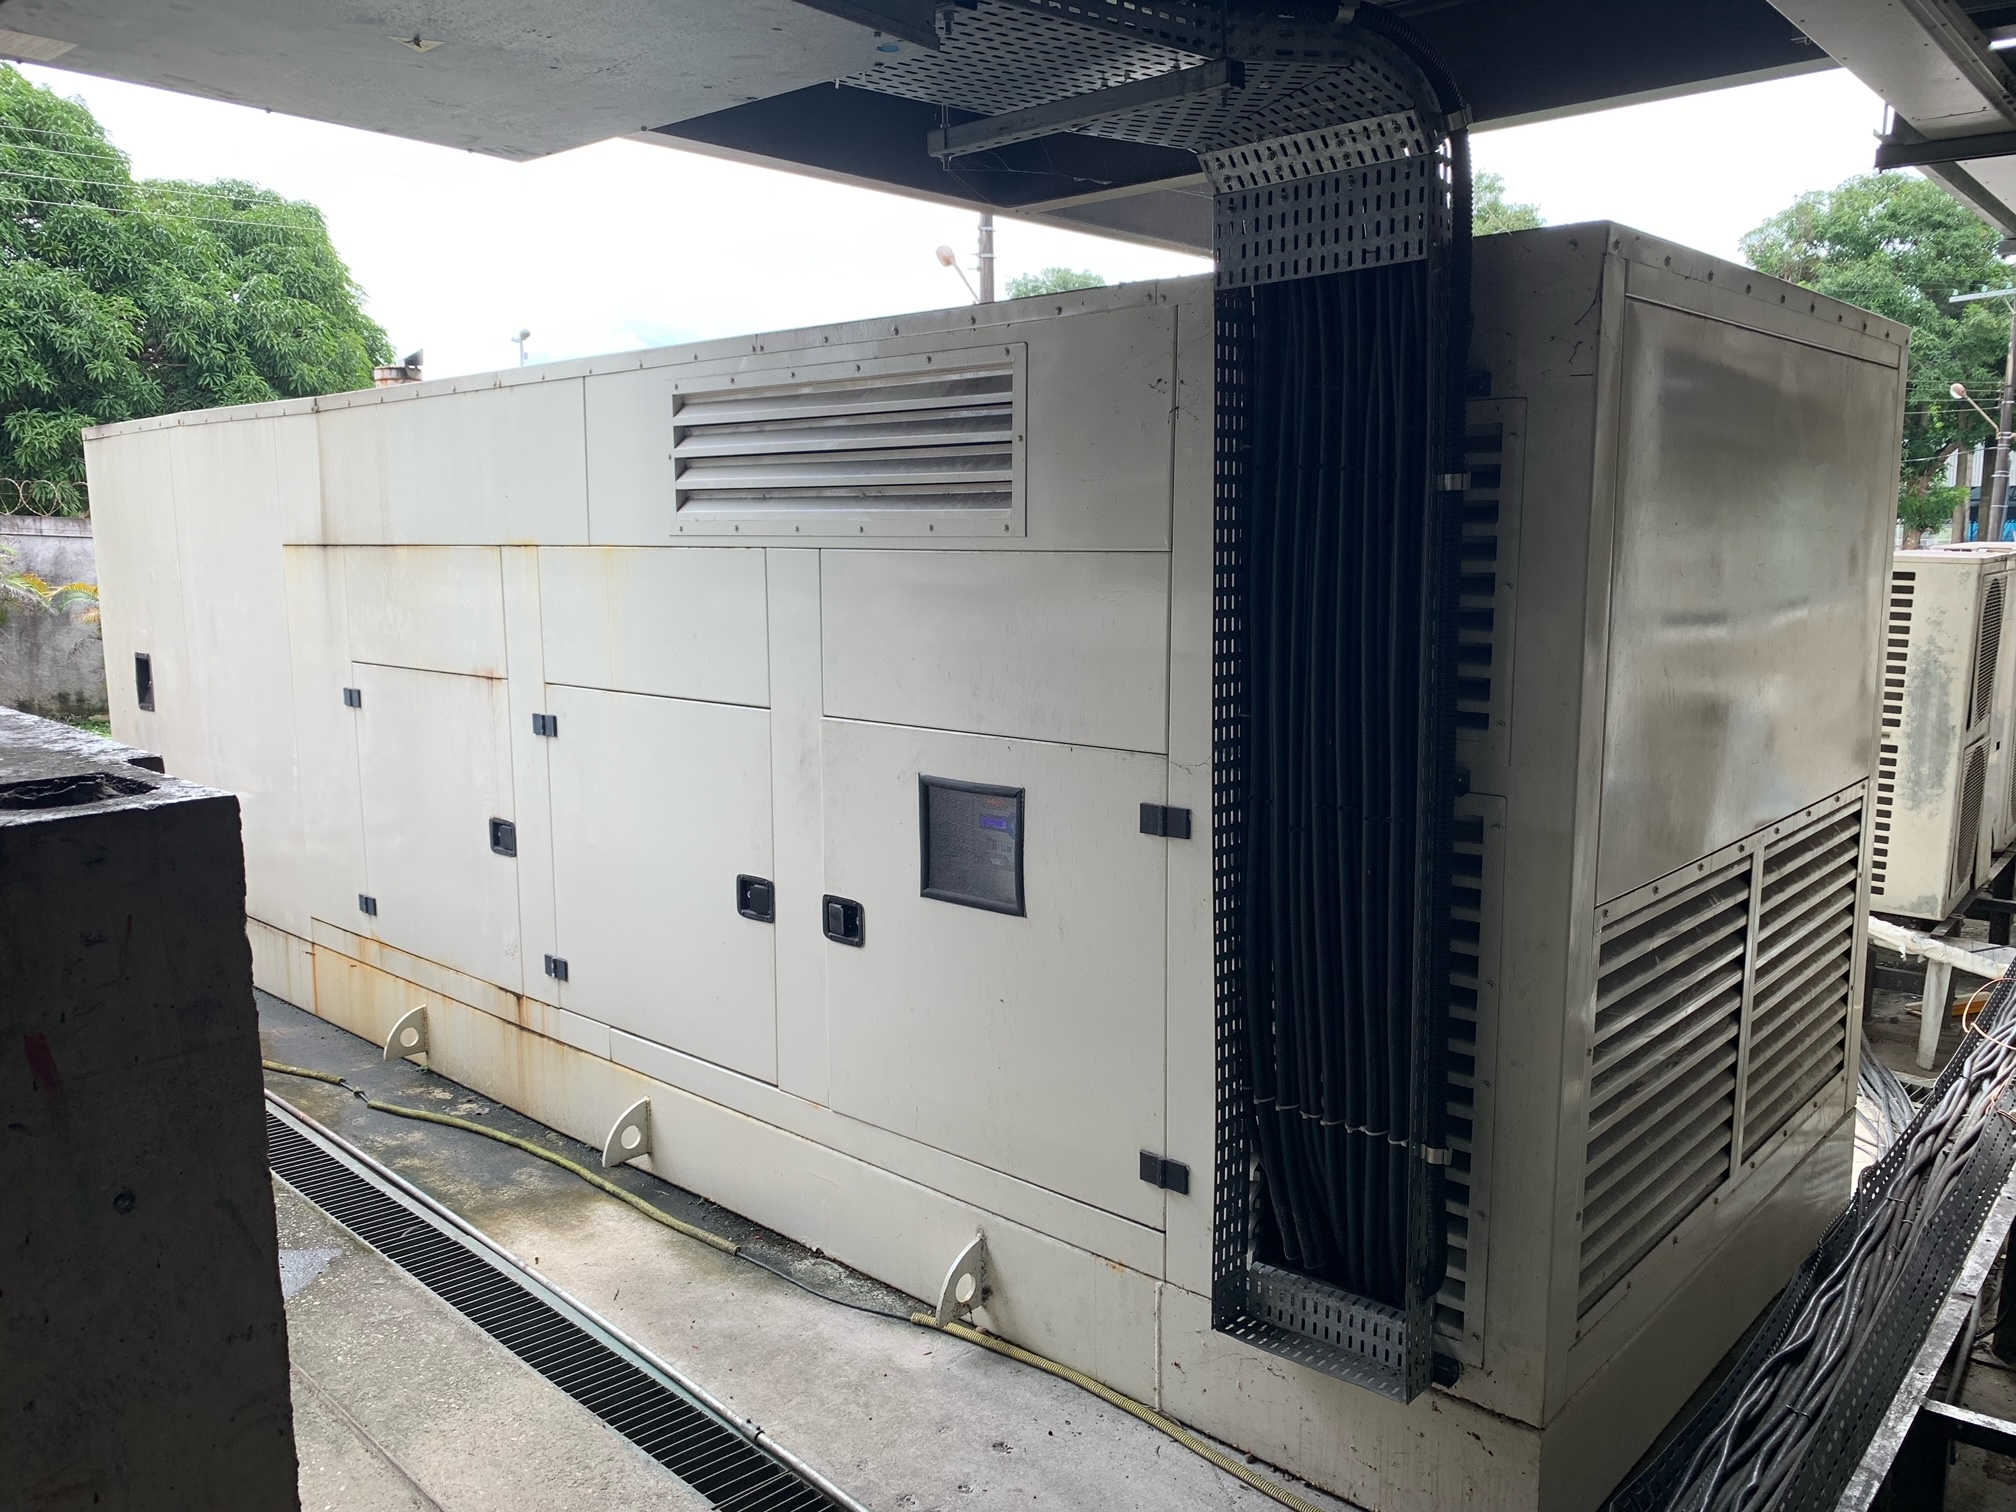
\includegraphics[width=.9\textwidth]{Figuras/gerador_750.jpeg}
            \vspace*{\fill} 
            \begin{quote} 
            \centering 
            Fonte: própria.
            \end{quote}
            \vspace*{\fill}
			\label{fig:gerador750}
\end{center}
\end{figure}

\subsubsection{Características de utilização}

\subsection{Grupo gerador prédio anexo}

\begin{figure}[H]
\begin{center}
			\caption{Grupo gerador prédio anexo de 450 kVA}
			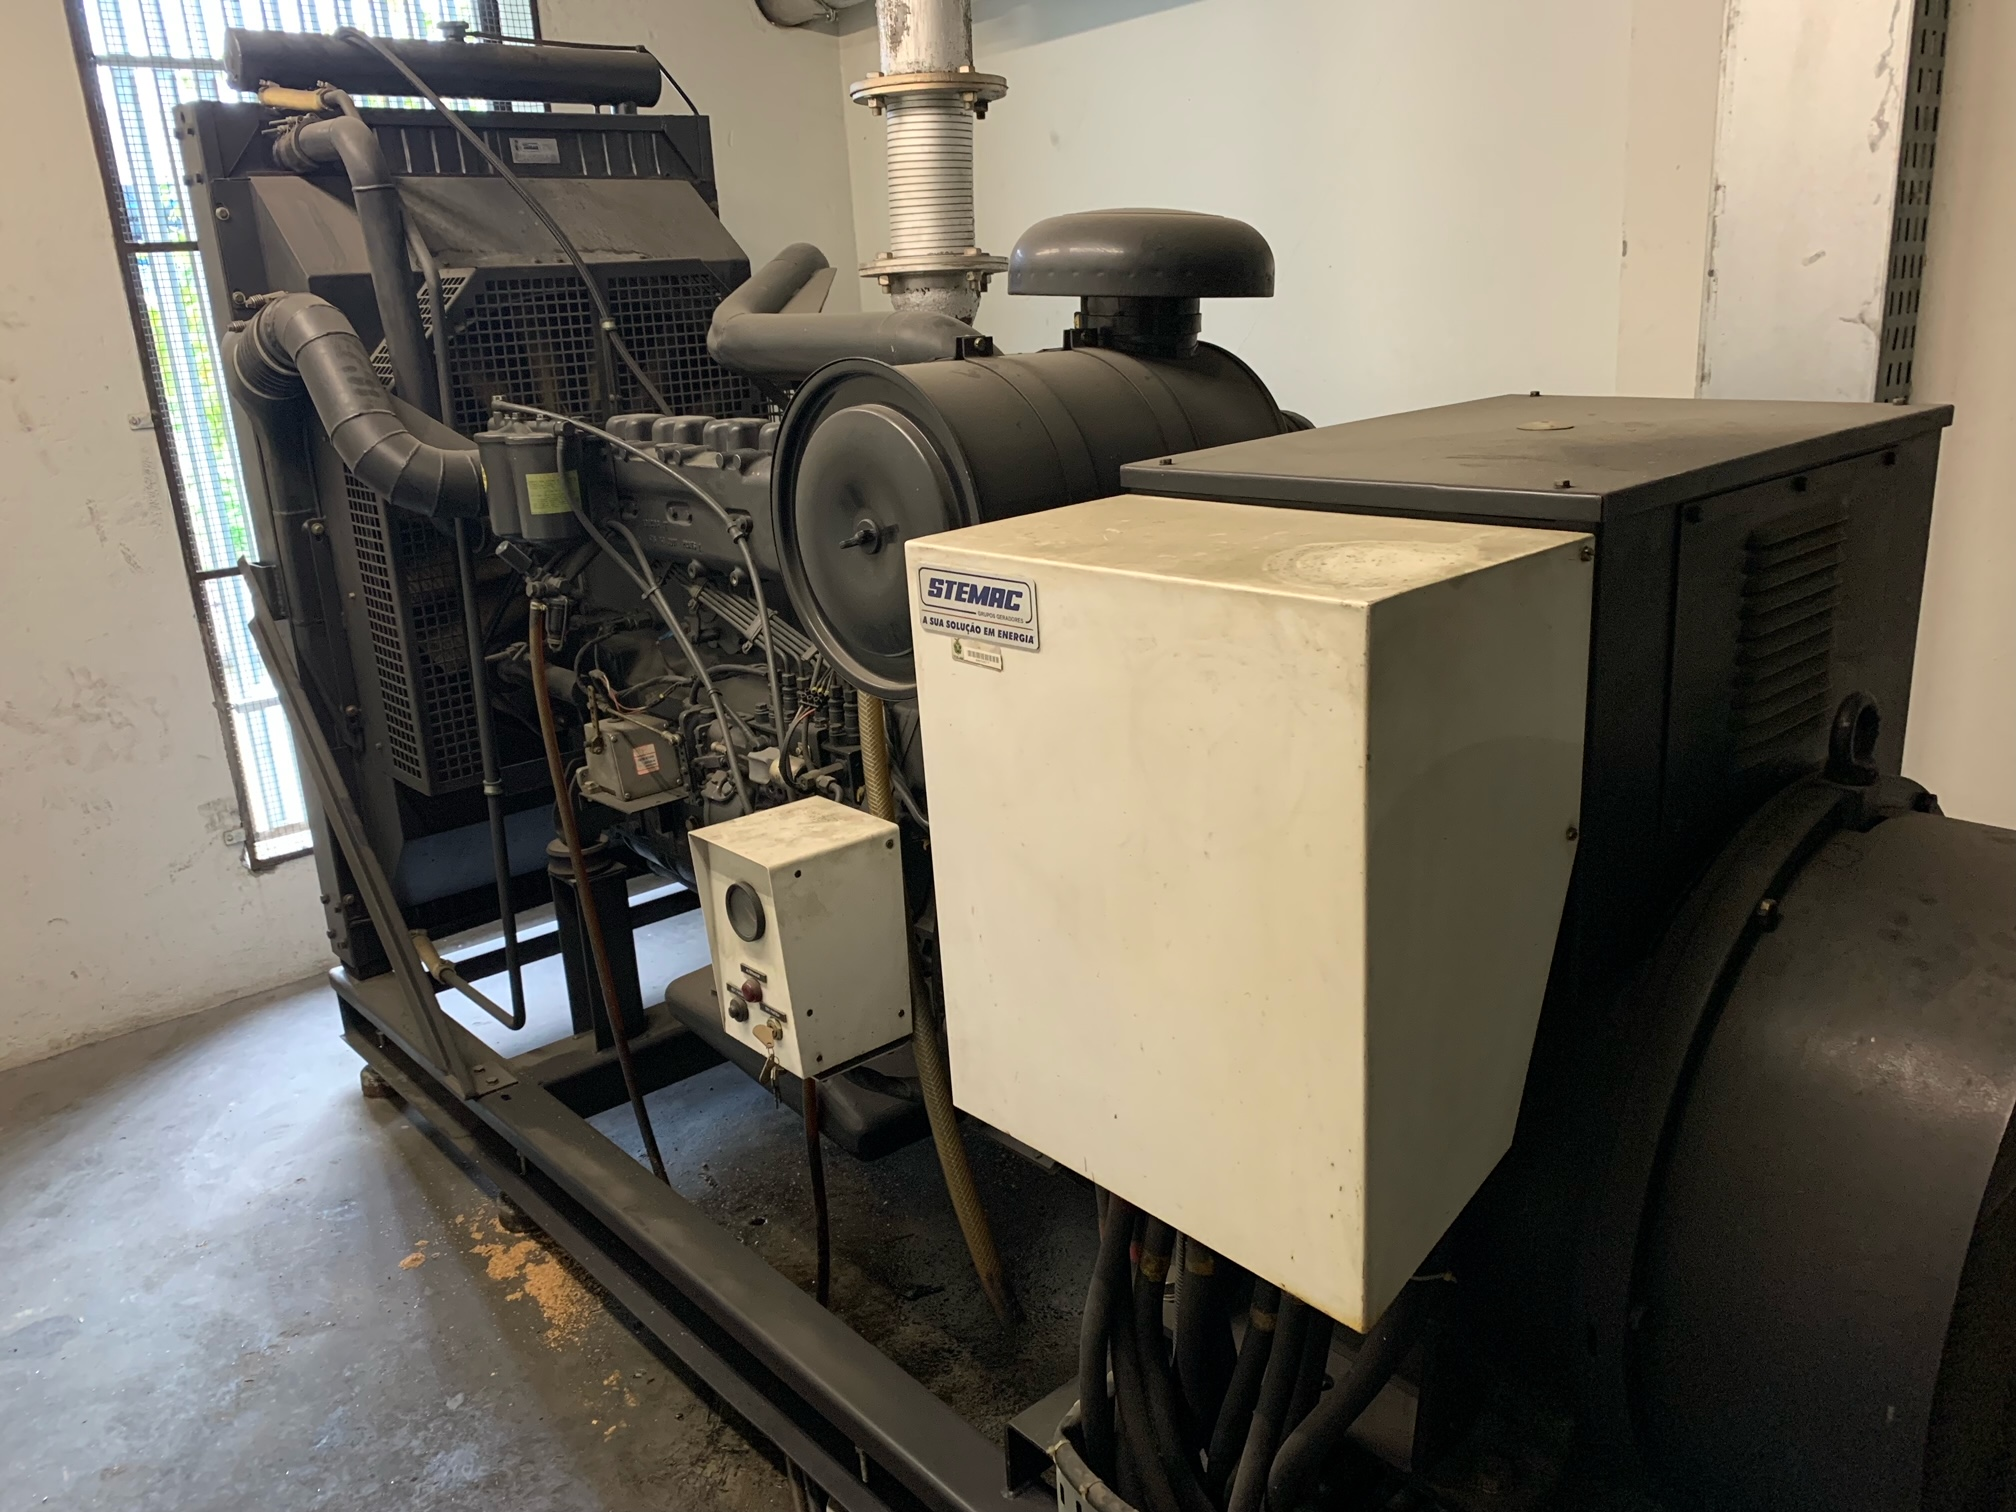
\includegraphics[width=.9\textwidth]{Figuras/gerador_450.jpeg}
            \vspace*{\fill} 
            \begin{quote} 
            \centering 
            Fonte: própria.
            \end{quote}
            \vspace*{\fill}
			\label{fig:gerador750}
\end{center}
\end{figure}

\section{ANÁLISE DE CARGA DA INSTALAÇÃO}

\hspace*{0.8cm} Este capítulo aborda a análise do das características de consumo. O diagrama esquemático deste sistema está exposto na  Figura \ref{fig:dia}. Deste diagrama, tem-se os eletrodos, que estão conectados no paciente; o cir\-cuito de aquisição para tratar e acomodar o sinal enquanto o MCP3008 é utilizando como conversor analógico/digital e se conecta com o Raspberry Pi 3 através da porta SPI. Ambos estão configurados para transmitir o sinal ECG. O sistema é iniciado com o pedido realizado pelo usuário, utilizando a arquitetura cliente-servidor presente nos computadores. Internamente o cliente
faz a requisição ao servidor presente no Raspberry Pi 3 e o interpreta, utilizando a rede Wi-Fi como meio de comunicação, realizando a leitura de dados da porta do MCP3008, a qual está conectada com o circuito de aquisição e por fim, o cliente recebe as amostras, fornecida pelo o servidor. \textcolor{red}{há extra "espaços"...verifique isso....acho que vc poderia quebrar esse para em dois e explicar um pouco melhor}


\begin{figure}[H]
\begin{center}
			\caption{Diagrama Esquemático do Sistema Proposto}
			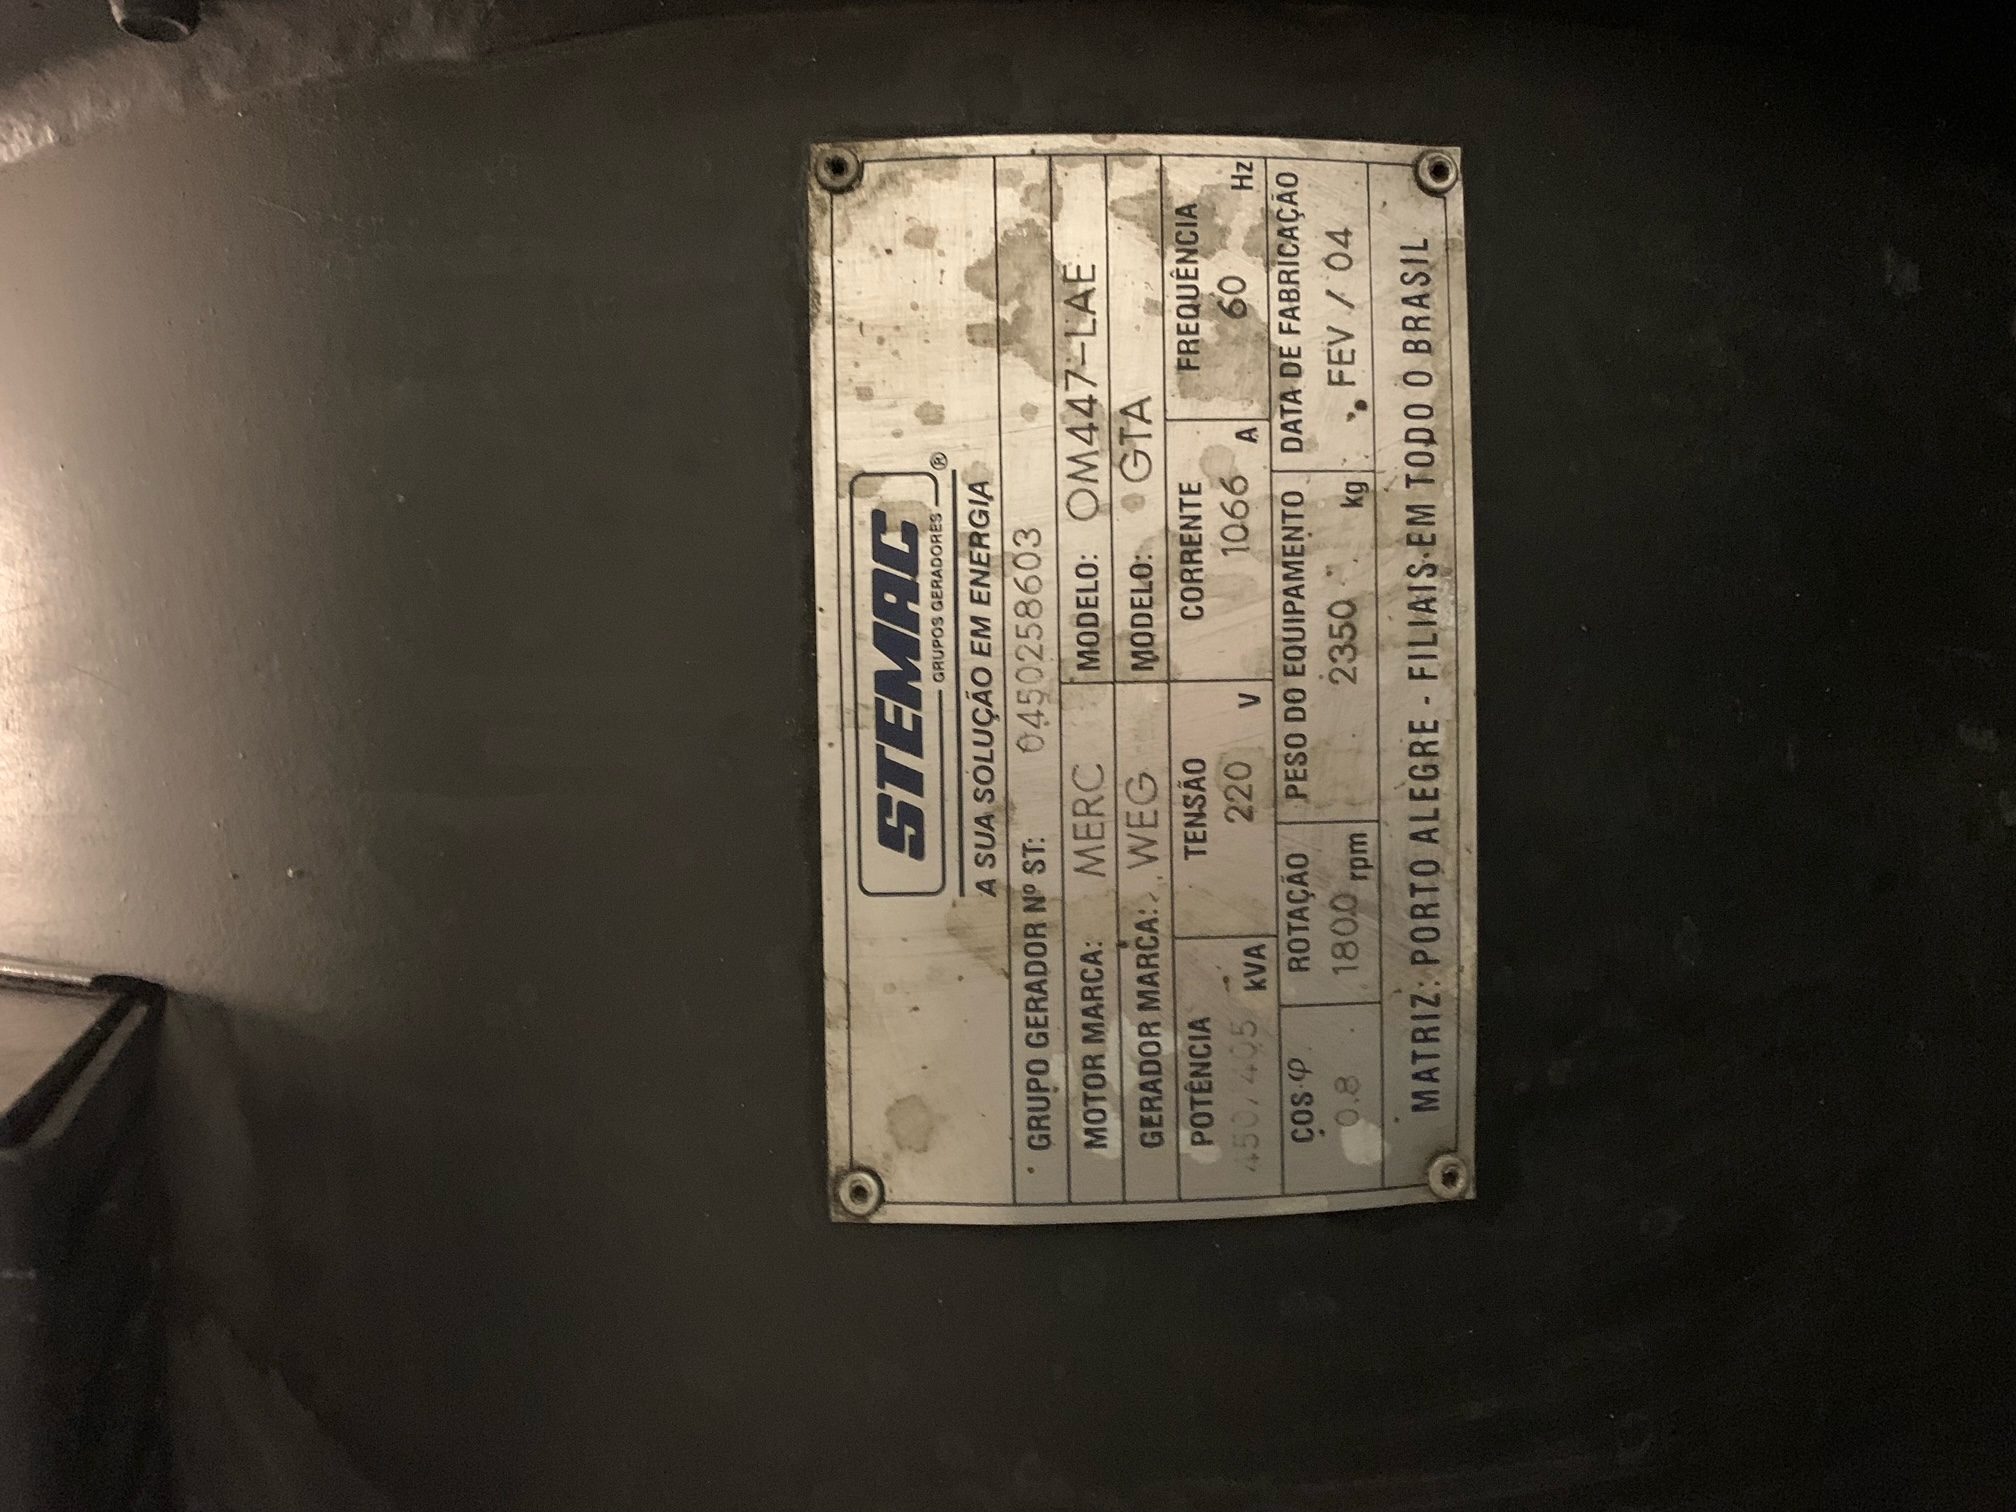
\includegraphics[width=.8\textwidth]{Figuras/info_gerador_450.jpeg}
            \vspace*{\fill} 
            \begin{quote} 
            \centering 
           Fonte: {Elaborada pela autora}
            \end{quote}
            \vspace*{\fill}
			\label{fig:dia}

\end{center}
\end{figure}



\subsection{DESENVOLVIMENTO DO HARDWARE}
\hspace*{0.8cm}Após a etapa de definição e aquisição de componentes que fazem parte da configuração do hardware, procedeu-se a implementação do circuito eletrônico em um protoboard, sendo que inicialmente foram realizados testes nos componentes eletrônicos. O primeiro teste consistiu na verificação dos sinais ECG utilizando a placa ECG AD8232, a qual foi alimentada com a tensão de 3,3V e utilizou o  pino GND para aterramento do sinal. Utilizou-se os pinos RA, LA e RL do simulador de sinais vitais HS-15 no modo ECG, conectado nos pinos RA, LA e RL da placa AD8232 com o intuito de analisar a forma de onda característica do sinal ECG, com o manuseio da ponta de prova do osciloscópio e assim analisar o sinal na tela do equipamento. \textcolor{red}{verifique os "espaços" novemente}
\newpage

\section{RESULTADOS}

\hspace*{0.8cm} Neste capítulo são abordados os resultados obtidos durante o desenvolvimento do trabalho de conclusão de curso. Destaca-se neste projeto dois resultados significativos, um deles é o protótipo físico desenvolvido, apresentado na Figura \ref{fig:mama} e o outro resultado diz respeito as formas de ondas obtidas que compõe mo sinal de ECG, formando pela onda P, complexo QRS e onda T. \textcolor{red}{E O BAIXO CUSTO????}

Os componentes utilizados na montagem do protótipo são apresentados no capítulo 3. Após, as etapas de montagem, soldagem e configuração, realizou o acomodamento do sistema, para isso utilizou uma caixa patola deixando apenas um espaço destinado conexão do cabo-flat com os pinos do Raspberry e a entrada do cabo paiciente, destaca-se que esse tipo de caixa é amplamente utilizada para acabamento estético, proteção de circuitos. A Figura \ref{fig:mama}, representa o dispositivo final, disposto na caixa patola.




\begin{figure}[H]
\begin{center}
			\caption{Dispositivo final, disposto na caixa patola}
			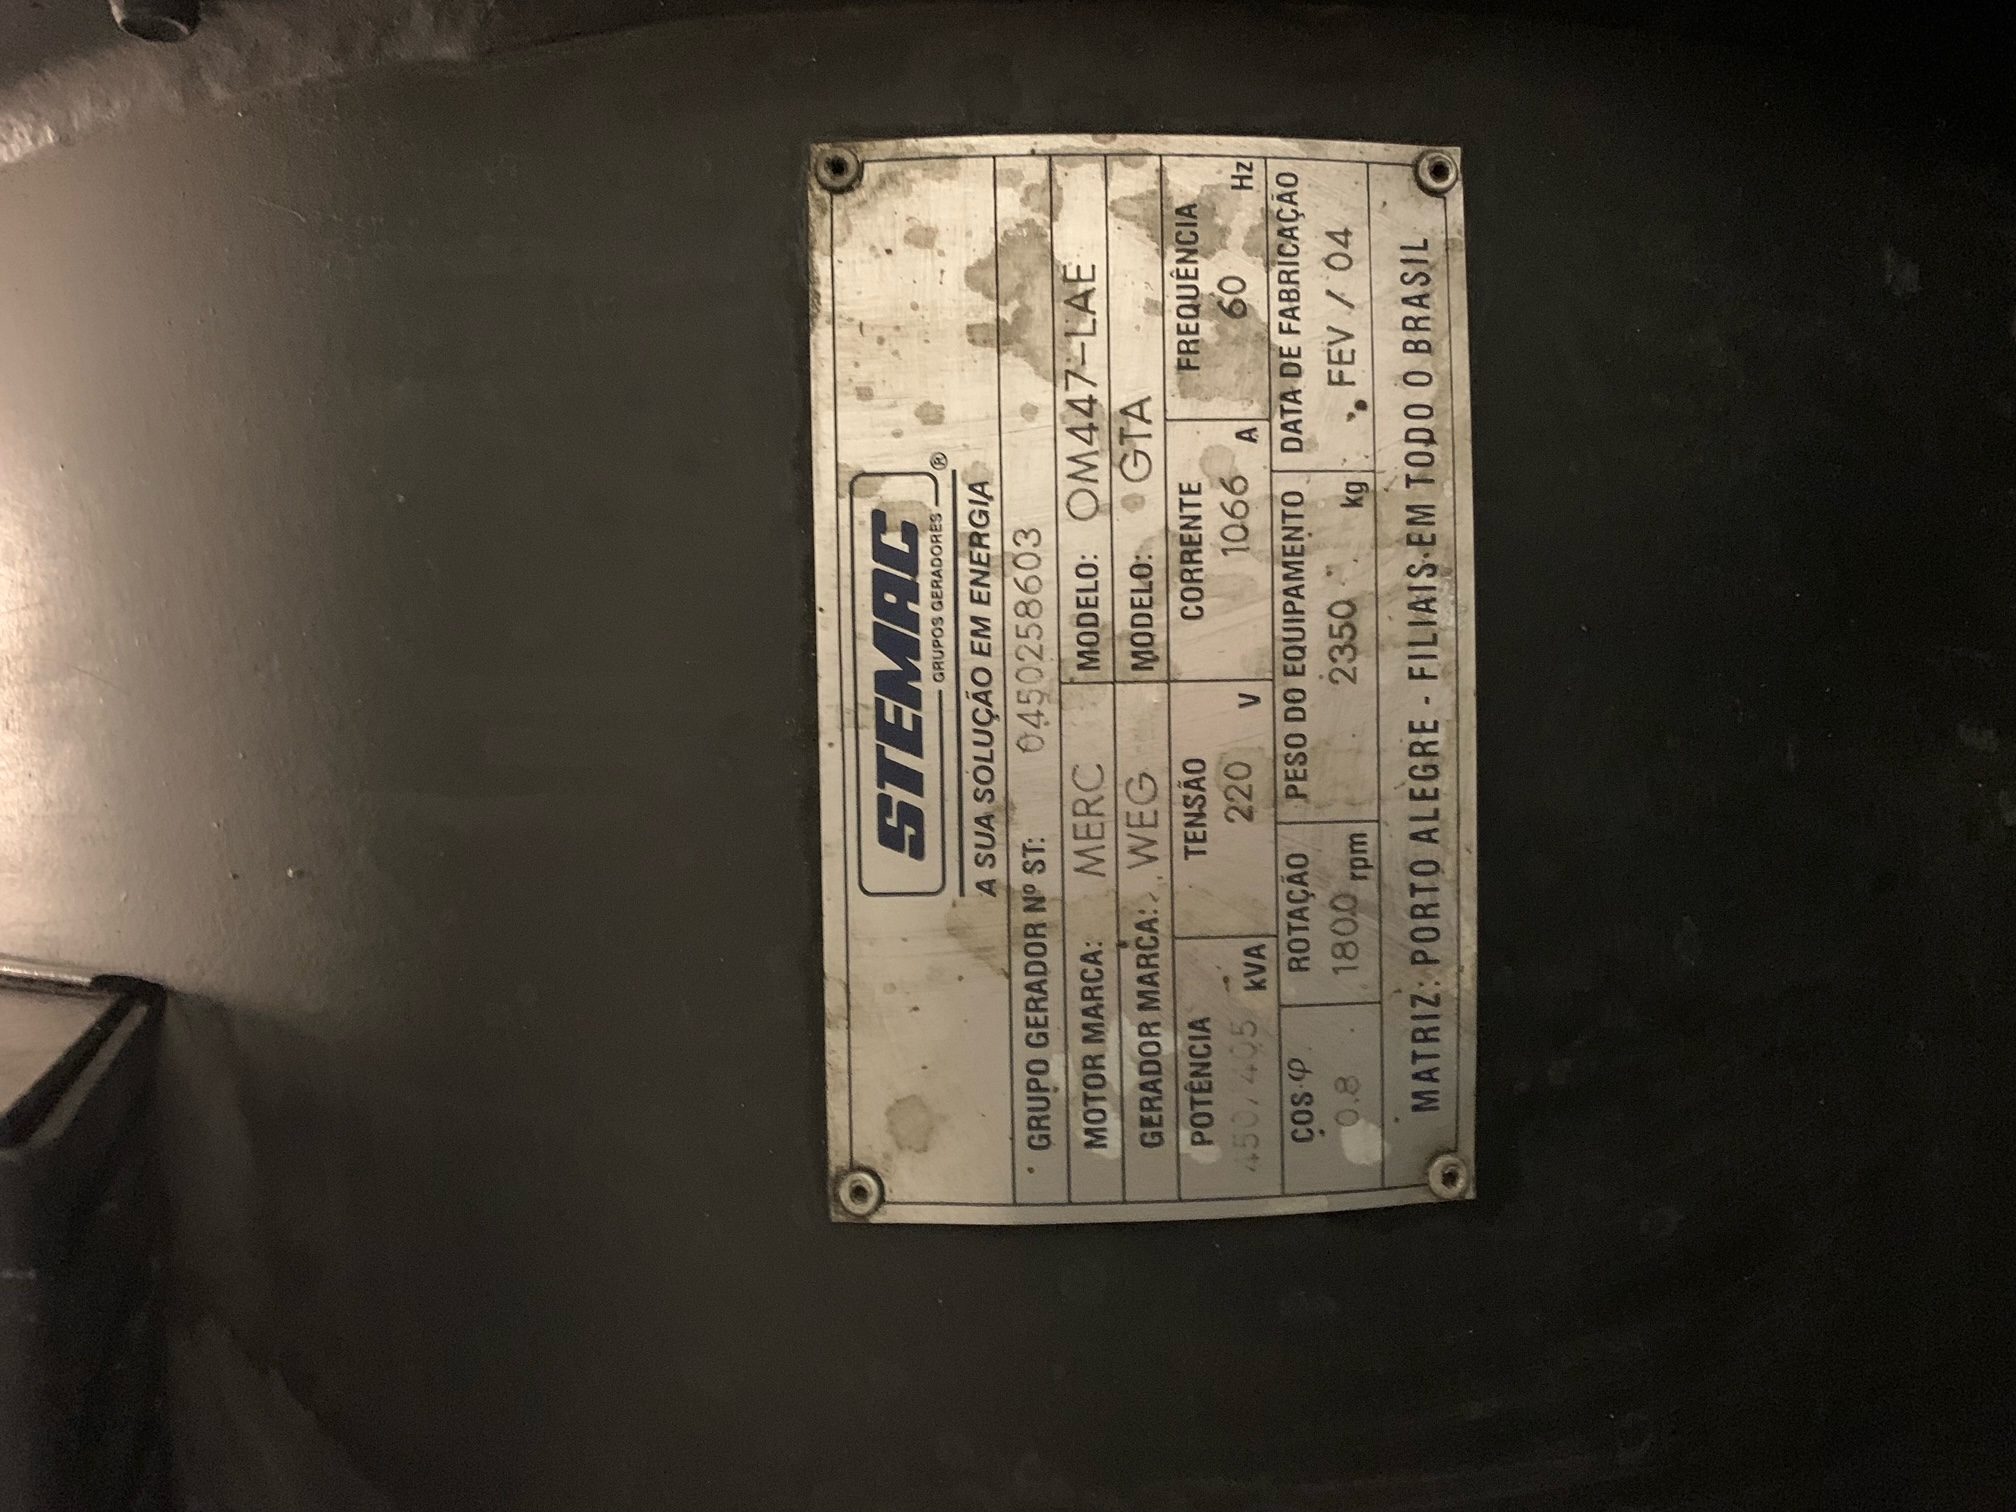
\includegraphics[width=.9\textwidth]{Figuras/info_gerador_450.jpeg}
              \vspace*{\fill} 
            \begin{quote} 
            \centering 
           Fonte: Elaborada pela autora
            \end{quote}
            \vspace*{\fill}
			
			\label{fig:mama}
\end{center}
\end{figure}
A utilização da placa baseada no CI AD8232 da Analog Device para obtenção dos sinais de ECG foi importante para eliminar as variáveis do processo de aquisição. O protótipo desenvolvido foi testado com o simulador de sinais vitais HS-15, e seus resultados foram comparados aos resultados da forma de onda padrão da segunda derivação eletrocardiográfica de um equipamento comercial modelo EP-12 da empresa Philips Dixtal \textcolor{red}{AQUI VAI UMA REF}.

A Figura \ref{fig:popi}, representa o sinal ECG simulado no equipamento eletrocardiógrafo EP12, o equipamente utiliza o mesmo modelo de simulador de sinais vitais utilizando neste trabalho. É possivel, analisar e verificar a semelhança com a o sinal exposto na Figura  \ref{fig:oscilo}.  O propósito deste projeto é fornecer com qualidade e parâmetros as formas de ondas característica do ECG. \textcolor{red}{MELHORE ESSA ULTIMA FRASE}

\begin{figure}[H]
\begin{center}
			\caption{Sinal de ECG simulado no EP12 Dixtal}
			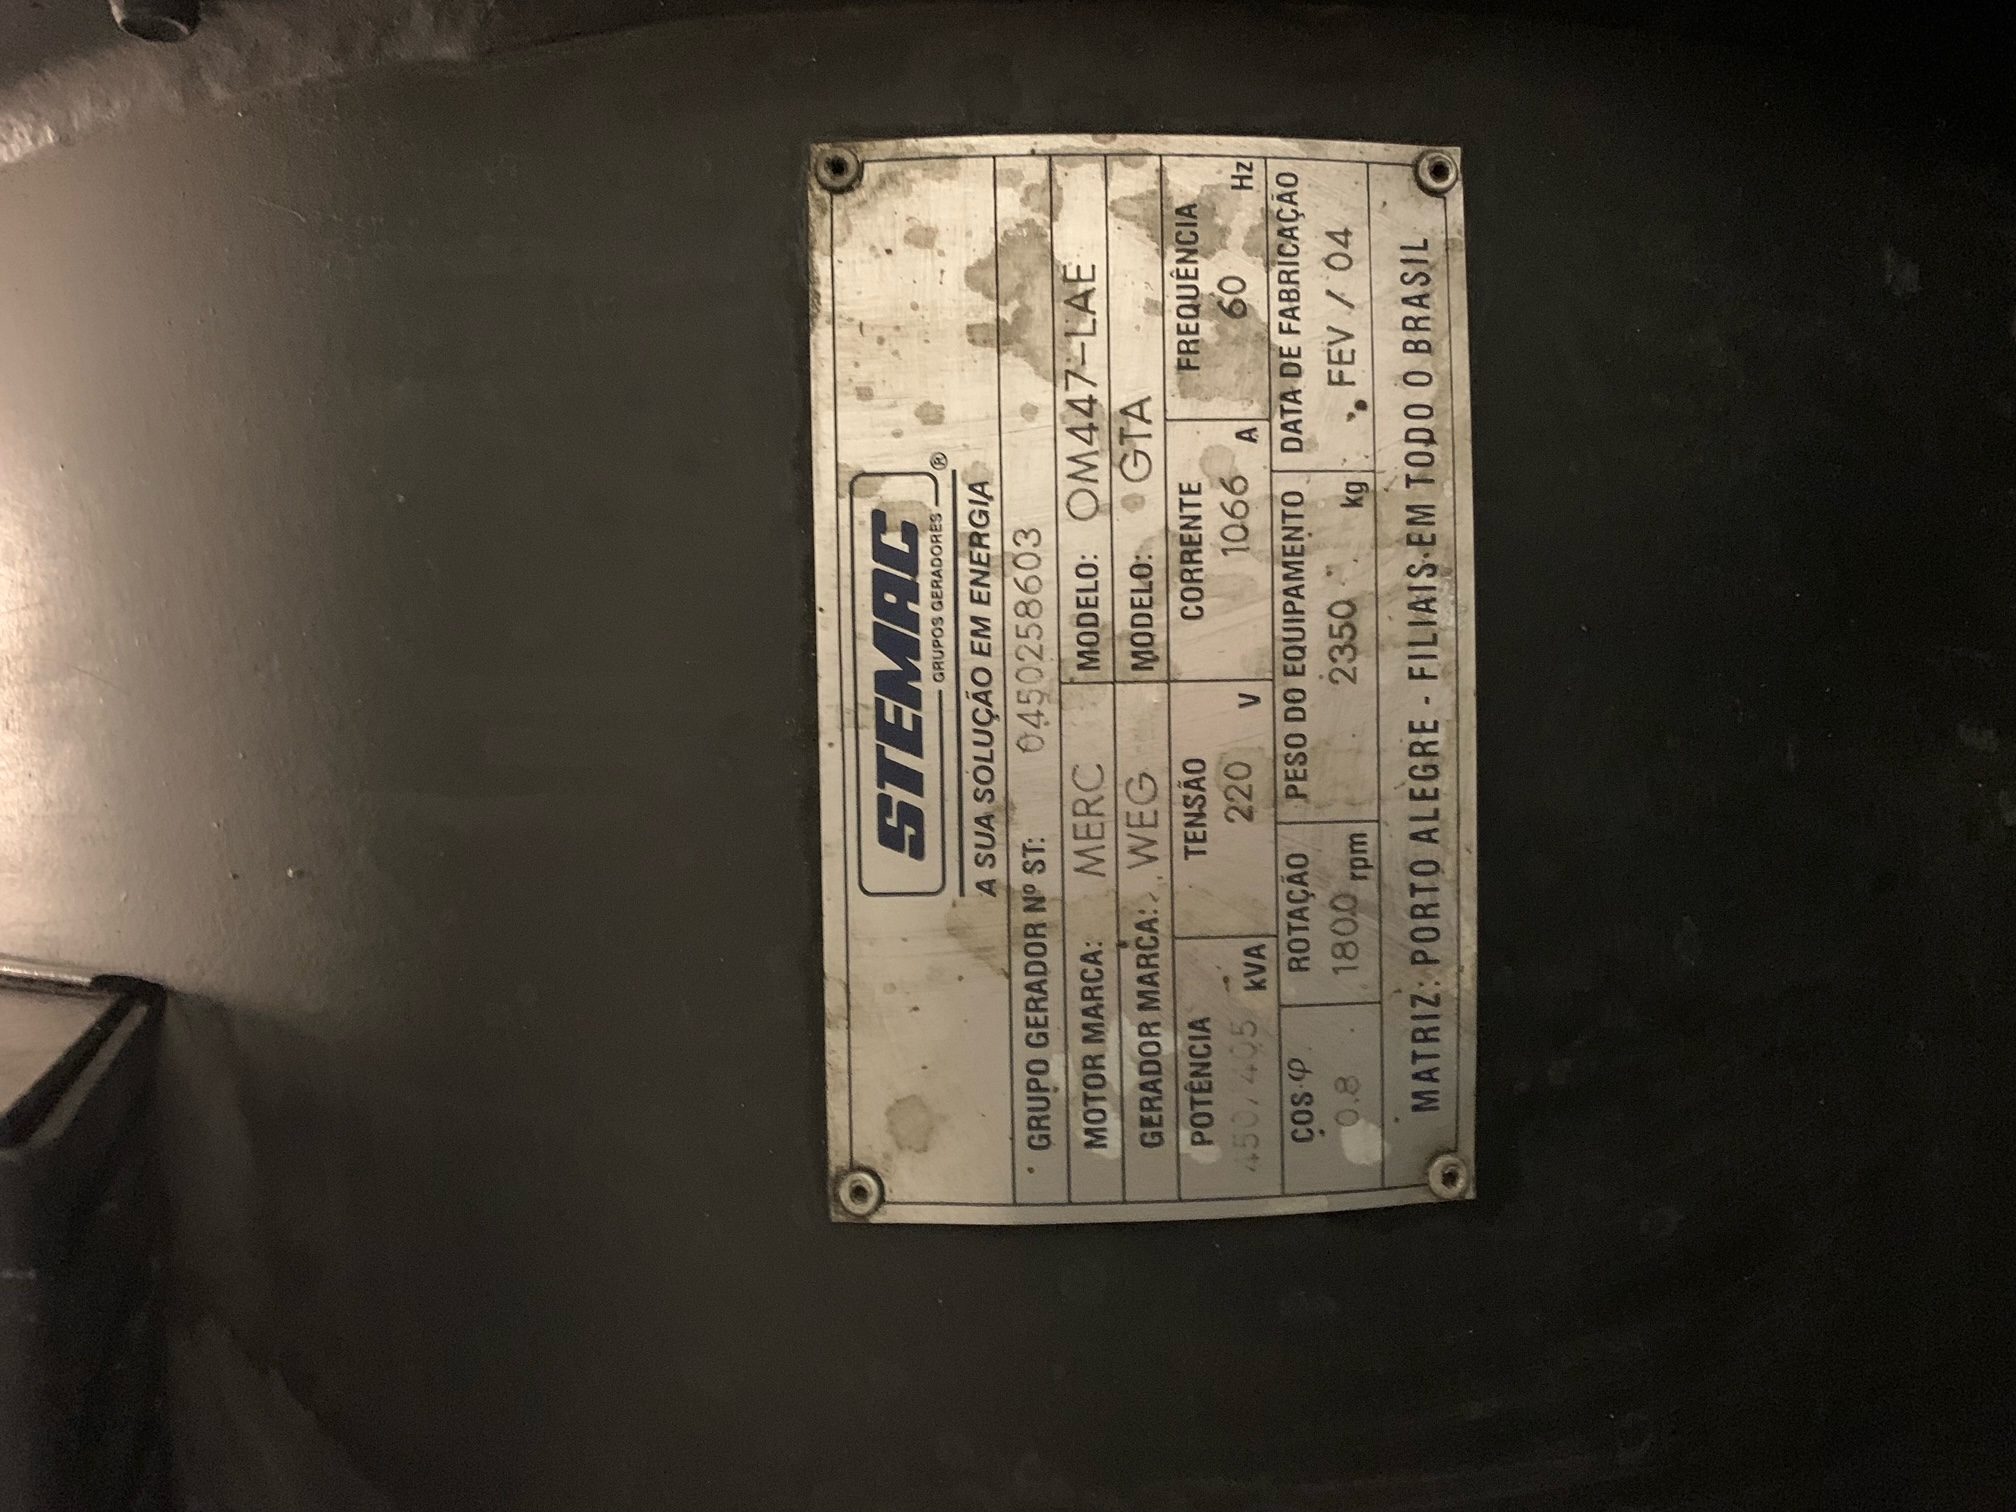
\includegraphics[width=.8\textwidth]{Figuras/info_gerador_450.jpeg}
              \vspace*{\fill} 
            \begin{quote} 
            \centering 
           Fonte: \cite{ronald}
            \end{quote}
            \vspace*{\fill}
			\label{fig:popi}
\end{center}
\end{figure}

A Figura \ref{fig:oscilo}, representa a forma de onda adquirida pelo o sistema de aquisição, utilizando o simulador para gerar sinais vitais e o oscilóscopio para análise. Este sinal é composto pela a onda p, complexo QRS e a onda T, característico da forma de onda do eletrocardiograma. \textcolor{red}{MELHORE ESSE PARA...ESCREVA MAIS OU MENOS ASSIM: NA FIGURA TAL, APRESENTA-SE A FORMA DE ONDA....SACOU??...EM GERAL, PROCURE ESCREVER ASSIM...OU SEJA, CORRIJA O RESTO...}

\begin{figure}[H]
\begin{center}
			\caption{Sinal do ECG obtido pelo o osciloscópio}
			\includegraphics[width=.9\textwidth]{Figuras/oscil.PNG}
             \vspace*{\fill} 
            \begin{quote} 
            \centering 
           Fonte: Elaborada pela autora
            \end{quote}
            \vspace*{\fill}
			\label{fig:oscilo}
\end{center}
\end{figure}

\hspace*{0.8cm}O Raspberry Pi 3 está sendo usado como servidor. O cliente solicita através do comando 'req' e para cada amostra é determinado um valor de acordo com o sinal fornecido pelo o simulador através da porta do mcp.read-adc(4), ou seja, a porta 4 do conversão analogico/digital. Essa leitura está sendo comprovado na Figura \ref{fig:kiki}.

\begin{figure}[H]
\begin{center}
			\caption{Amostragem Sinal do ECG}
			\includegraphics[width=.9\textwidth]{Figuras/json.PNG}
			              						\vspace*{\fill} 
            \begin{quote} 
            \centering 
           Fonte: Elaborada pela autora
            \end{quote}
            \vspace*{\fill}
			\label{fig:kiki}
\end{center}
\end{figure}

Os testes de transmissão e recepção do sinal utilizando a arquitetura cliente-servidor proposta foram realizados conectando os dispositivos através da rede Wi-fi do HUB. Com o resultado dessa arquitetura, tem-se a forma de onda utilizando o simulador de sinais vitais, conectado ao protótipo. Nestes testes, utilizou-se o simulador e foi variado a amplitude e o batimento por minuto.

A Figura \ref{fig:ecg2}, representa um resultado da arquitetura e o protótipo. A imagem representa o sinal ECG simulado, composto por 500 amostras de amplitude do sinal em determinado tempo. Esse sinal é composto inicialmente pela a onda P, complexo QRS e seguindo a onda T. 


\begin{figure}[H]
\begin{center}
			\caption{Sinal ECG simulado}
			\includegraphics[width=.8\textwidth]{Figuras/sinal.PNG}
                          						\vspace*{\fill} 
            \begin{quote} 
            \centering 
           Fonte: Elaborada pela autora
            \end{quote}
            \vspace*{\fill}
			\label{fig:ecg2}
\end{center}
\end{figure}
\begin{figure}[H]

\hspace*{0.8cm}Para a validação do sistema proposto, o usuário solicita através de comando utilizando o cliente, o qual requisita ao servidor usando topologia estabelicida, o qual faz a leitura de dados e a transfere para o servidor. A Figura \ref{fig:syst}, exibe o sistema em operação: uma tela está exibindo a resposta solicitada ao servidor, ou seja, o sinal ECG adquirido pelo sistema de aquisição utilizando sinais fornecido pelo o  simulador de sinais vitais e a outra tela, apenas faz a exibição da leitura do MCP3008.

\begin{center}
			\caption{Sistema em Operação}
			\includegraphics[width=.9\textwidth]{sist.PNG}
            	\vspace*{\fill} 
            \begin{quote} 
            \centering 
           Fonte: Elaborada pela autora
            \end{quote}
            \vspace*{\fill}
			\label{fig:syst}
\end{center}
\end{figure}

\newpage
\section{ANÁLISE ECONÔMICA E AMBIENTAL}


\newpage


% Uncomment the following two lines if you want to have a bibliography. Please do not forget to add an entry to your bibliography and reference it by using the \cite{} command
%\bibliographystyle{alphadin}
\providecommand*{\refname}{}
\renewcommand*{\refname}{\begin{center}\textbf{REFERÊNCIAS}\end{center}}

\newpage
\vspace*{4cm}
%\providecommand{\bibname}{}
%\renewcommand{\bibname}{\begin{center}\textbf{REFERÊNCIAS}\vspace{48pt}\end{center}}

\pagestyle{empty}
\pagestyle{myheadings}

%\bibliographystyle{alpha}

\addcontentsline{toc}{section}{REFER\^ENCIAS}
\bibliography{bibliografia}

% End of the document
\end{document}
